%%%%%%%%%%%%%%%%%%%%%%%%%%%%%%%%%%%%%%%%%%%%%%%%%%%%%%%%%%%%%%%%%%%%%%%%%%%%%%%%
%\documentclass[12pt,papel,twoside]{ibtesis}
\documentclass{ibtesis}

% \documentclass[12pt,papel,singlespace,oneside]{ibtesis}
% \documentclass[12pt,papel,preprint,singlespace,oneside]{ibtesis}

%%%%%%%%%%%%%%%%%%%%% Paquetes extra %%%%%%%%%%%%%%%%%%%%%%%%%%%%%%%%%%%%%%%%%%%
% Por conveniencia: aqu\'{\i} puede cargar todos los paquetes y definir los comandos 
% que necesite
\usepackage{ibextra}
\usepackage[utf8]{inputenc}
\usepackage{subcaption}  % Enable figure captions or figure notes
\usepackage{float}
\usepackage{nicefrac}
\usepackage{mathtools}
\usepackage{textcomp}

\usepackage{amsfonts}

\newcommand{\done}{\item[\checkmark]}
%%%%%%%%%%%%%%%%%%%%%%%%%%%%%%%%%%%%%%%%%%%%%%%%%%%%%%%%%%%%%%%%%%%%%%%%%%%%%%%%
%%%%%%%%%%%%%%%%%%%%% Informacion sobre la tesis %%%%%%%%%%%%%%%%%%%%%%%%%%%%%%%
\title{Informe de Avance}
\author{Evelyn~G.~Coronel}
\director{Dra.~Silvia Mollerach}
%\codirector{Dr.~J.~Otro m\'{a}s}b
\carrera{Tesis de Maestría en Ciencias F\'{\i}sicas}
\grado{Maestrando}
\laboratorio{Partículas y Campos -- Centro At\'{o}mico Bariloche}
\jurado{Dr.~Diego~Harari (Instituto Balseiro)}

\palabrasclave{Rayos Cósmicos, Análisis de datos, Instituto Balseiro}
%\keywords{Cosmic Rays, Data Analysis, Balseiro Institute}
%\neembaeguasu{Mba'e michĩ yvágagui ouva, Mbo'ehaoguasu Balseiro}
% Si queremos poner la fecha manualmente:
% \date{Diciembre de 2099}

%%%%%%%%%%%%%%%%%%%%%%%%%%%%%%%%%%%%%%%%%%%%%%%%%%%%%%%%%%%%%%%%%%%%%%%%%%%%%%%%
%\titlepagefalse 
%%%%%%%%%%%%%%%%%%%%%%%%%%%%%%%%%%%%%%%%%%%%%%%%%%%%%%%%%%%%%%%%%%%%%%%%%%%%%%%%


% \setcounter{tocdepth}{4}
% \setcounter{secnumdepth}{4}
\begin{document}

\begin{preliminary}

%%% \'{I}ndices %%%%

\begin{abreviaturas}

\begin{tabular}{l l}
CR: 		& Rayos cósmicos  (\emph{Cosmic Rays}) \\
%CMB: 		& Radiación Cósmica de Fondo (\emph{Cosmic Microwave Background})\\
%FD: 		& Detector de Fluorescencia (\emph{Fluorescence Detector}) \\
SD: 		& Detector de Superficie (\emph{Surface Detector})  \\
%WCD: 		& Detector de radiación Cherenkov de agua\\
EAS: 		& Lluvia Atmosférica Extendida  (\emph{Extensive Air Shower})    \\
%VAOD: 		& Profundidad atmosférica óptica vertical (\emph{Vertical Atmosferic Optical Depth})\\
%CLF:		& \emph{Central Laser Facility}\\
%XLF:		& \emph{eXtreme Laser Facility}\\
%X$_{max}$: & Profundidad atmosférica del máximo de la lluvia \\
%LDF: 		& Función de Distribución Lateral (\emph{Lateral Distribution Function}) \\
S(1000): 	& Señal a 1000\,m del núcleo de la lluvia y al nivel del suelo \\
S(1000)$_w$:& Señal de S(1000) corregida por la modulación del clima. \\
%CIC: 		& Corte de Intensidad Constante (\emph{Constant Intensity Cut}) \\
S$_{38}$: 	& Señal a 1000\,m del núcleo y al nivel del suelo si el ángulo cenital del evento fuera de $38^o$\\
S$_{38,w}$: & Señal S$_{38}$ corregida por la modulación del clima \\
eV: 		& electrón Voltio, $1\,$eV$= 1.602\times 10^{-19}\,$J \\
EeV: 		& $1\,$EeV$=10^{18}\,$eV\\
%PMT: 		& Tubo fotomultiplicador (\emph{Photo-Multiplier Tube})\\
%VEM: 		& Muón vertical equivalente (\emph{Vertical Equivalent Muon})\\
ICRC: 		& Conferencia Internacional de Rayos Cósmicos (\emph{International Cosmic Ray Conference})\\
\end{tabular}
                     %Abreviaturas
\end{abreviaturas}

	\tableofcontents                %\'{I}ndice
	\listoffigures                  %Figuras
	%\listoftables                  %Tablas

	%\begin{resumen}%
Cuando un rayo cósmico interactúa con una molécula en la parte superior de la atmósfera, se inicia un proceso en el cual se generan otras partículas secundarias. Este proceso es conocido como lluvia atmosférica extendida. Estas lluvias pueden ser detectadas sobre la superficie de la Tierra mediante varios experimentos. Este trabajo utiliza los datos recolectados por los detectores de superficie separados en 1500\,m entre sí del Observatorio Pierre Auger durante los años 2005-2020. 

Se estudian eventos obtenidos mediante distintos algoritmos de adquisición de datos. El \emph{Disparo Estándar} que alcanza eficiencia completa para eventos asociados a rayos cósmicos de energía mayor a $3\,$EeV, y el \emph{Todos los Disparos} llega a detectar, con una eficiencia del 100\%, eventos por encima de $1\,$EeV. El primer disparo contiene eventos registrados desde el año 2005 y el segundo disparo empezó funcionar desde el 2013. 

Las condiciones atmosféricas como la presión (P), la temperatura (T) y la densidad ($\rho \propto \nicefrac{P}{T}$) afectan el desarrollo de la lluvia a través de la atmósfera. Las variaciones de estas condiciones inducen una modulación en la señal producida en los detectores por un rayo cósmico de una dada energía. Mediante un estudio hecho por la Colaboración sobre eventos del Disparo Estándar, se corrigió el efecto de esta modulación en la estimación de la energía de los rayos cósmicos medidos por el Observatorio. En este trabajo extendimos el periodo de tiempo analizado de esta modulación, y se observó que los parámetros obtenidos son comparables con la reconstrucción oficial. También se estudia la modulación en los datos de Todos los Disparos, y se realiza una corrección sobre el mismo conjunto de datos usando los parámetros obtenidos por este trabajo.

Se  estudian las modulaciones en distintas frecuencias mediante el análisis en Rayleigh, y se propone una variable generalizada para hacer un barrido en frecuencias con el método de East-West. Se obtienen resultados de la modulación en ascensión recta para distintos rangos de energía y se comparan con resultados reportados por la Colaboración Pierre Auger.

\end{resumen}


% \begin{nemombyky}%
% Mbyjakua\'ape (\emph{astronomía} karaiñe'\~eme) ojeikuaase mba\textquotesingle e oik\'ova umi mba\textquotesingle e  michĩ yv\'agagui o\'uva (\emph{rayos cósmicos} karaiñe'\~eme) oguah\~evove amo yvatetépe (\emph{atmósfera} karaiñe'\~eme). Ombok\'aramo tuminguaave\textquotesingle \~yty (\emph{conjunto de átomos o molécula}  karaiñe'\~eme ) yvatetépe oĩva, oñepyr\~u ojapo het\~a umi tuminguaave\textquotesingle \~yjokaku\'era (\emph{partículas}  karaiñe'\~eme ) op\'arupi. Ko\textquotesingle a       ha\textquotesingle e  h\'ina peteĩ ama guasu tuminguaave\textquotesingle \~yjoka rehegua ( \emph{lluvia atmosf\'erica extendida} karaiñe'\~eme). Umi ama guasuku\'era tuichaterei ha ikatu eñeña\textquotesingle ã yvy ári op\'arupi. Mend\'osape oĩ peteĩ mba\textquotesingle etuicha h\'erava \emph{Pierre Auger} Mbyjañama\textquotesingle \~eha\~gua (\emph{Observatorio Pierre Auger}) oña'\~ava ko ama. Ko\textquotesingle  ape romba\textquotesingle  ap\'ota umi ama ko mbyjañama\textquotesingle \~eha\~gua oña\textquotesingle \~ava\textquotesingle  kue 2005-guive 2018-peve. Mba\textquotesingle \'eichapa umi amaku\'era oguah\~e yvy \'ari ikatu ojuavy hakúramo (T, \emph{temperatura} karaiñe\textquotesingle \~eme) tér\~a  poh\'yiramo pe pytundyry mbyjañama\textquotesingle \~eha\~gua áripe ($\rho$, \emph{densidad} h\'erava karaiñe\textquotesingle \~eme). Ko mbyjañama'\~eha\~gua ojapova\textquotesingle ekue peteĩ tembiapo ha ko\textquotesingle ape rojapojey up\'eva roikuaaha\~gua umi papapo oñenoh\~eva\textquotesingle ekue oiko gueteri ko'\~anga peve, ha rotopa kóva oikópa añetete.
% \end{nemombyky}



%%% Local Variables: 
%%% mode: latex
%%% TeX-master: "template"
%%% End: 


\end{preliminary}


\chapter{Introducción}
\graphicspath{{0_Introduccion/}}
% INTRODUCCION

La parte superior de la atmósfera terrestres esta siendo constantemente bombardeada con partículas de energía del orden de los $10^10\,$eV para arriba. Estas partículas son conocidas como rayos cósmicos (RC) y han sido medidas desde mediados del año 1961 \cite{linsley1961extremely}, pero los mecanismos que las producen y sus zonas donde se originan siguen siendo investigadas (citar experimentos). %La información sobre su origen puede ser obtenidas mediante el estudio de sus direcciones de arribo, también mediante el espectro de energía y sus composición de masa (cite y cite), aunque se espera que la evidencia más directa de la localización de su origen sea mediante  el estudio de la distribución de  las direcciones de arribo. La búsqueda de anisotropías a grandes escalas angulares suelen ser hechas sobre las irregularidades de la distribución de eventos en ascensión recta $\alpha$ ya que el arreglo principal tiene una exposición en función de este coordenada es casi constante \cite{referencia_anis}.


Por encima de una energía de $\sim10^14$EeV, los RCs que llegan a la atmósfera producen cascadas de partículas secundarias que pueden llegar hasta la superficie  de la Tierra. Estas cascadas son conocidas como lluvia atmosférica extendida o EAS. Estas lluvias contienen un componente electromagnética, que consiste en electrones, positrones y fotones, y una componente muónica que pueden ser medidas usando detectores de partículas sobre la superficie. Las partículas cargadas también pueden excitar moléculas de nitrógeno en el aire que producen fotones de fluorescencia, que pueden ser observadas por telescopios durante noches claras.


El observatorio Pierre Auger está ubicado en la ciudad de Malargüe, provincia de Mendoza. El mismo fue construido para detectar las partículas secundarias de la EAS producidas por RCs con energía por encima de $0.1\,$EeV. El observatorio posee un sistema híbrido de detección, ya que combina un arreglo de detectores de partículas superficiales y un conjunto de telescopios que detectan los fotones de fluorescencia.


Los análisis presentados en este trabajo fueron realizados con los eventos obtenidos por $\sim 1600$ detectores Cherenkov, dispuestos en una superficie de $\sim 3000\,\text{km}^2$ en un arreglo de forma hexagonal a una distancia de $1500\,$m entre sí, esta disposición de tanques se menciona como \textit{arreglo principal}. Cada detector en un tanque cilindro con 12 toneladas de agua ultra-pura de $1.2\,$m de alto, en la parte superior del tanque tiene 3 foto-multiplicadores que monitorean la radiación Cherenkov en el agua. El conjunto del tanque con la electrónica de detector se menciona durante el trabajo como \textit{Surface Detector} o \textit{SD}.  Cada detector está midiendo constantemente los fotones en el agua. Muchos de los estos fotones son producidos por ruido y otros por partículas secundarias de una EAS. Los SDs cuentan con algoritmos o reglas para discernir ruido de un evento causado por un rayo cósmico, estos son los algoritmos de disparo (cite).


\section{Acerca de todos los disparos del SD}

A medida que los tanques pasan más tiempo midiendo, también van perdiendo sensibilidad a los eventos de bajas energías. Esto es una desventaja del disparo estándar en los SDs en el rango $1\,$EeV - $2\,$EeV. En la Fig.\ref{fig:futuro}, para los datos presentados en el ICRC 2019, se observa como la energía media de los eventos para distintos rangos de tiempo va aumentando con el tiempo. Además que la proporción de eventos por debajo de $3\,$ EeV disminuye. 

\begin{figure}[H]
	\centering
	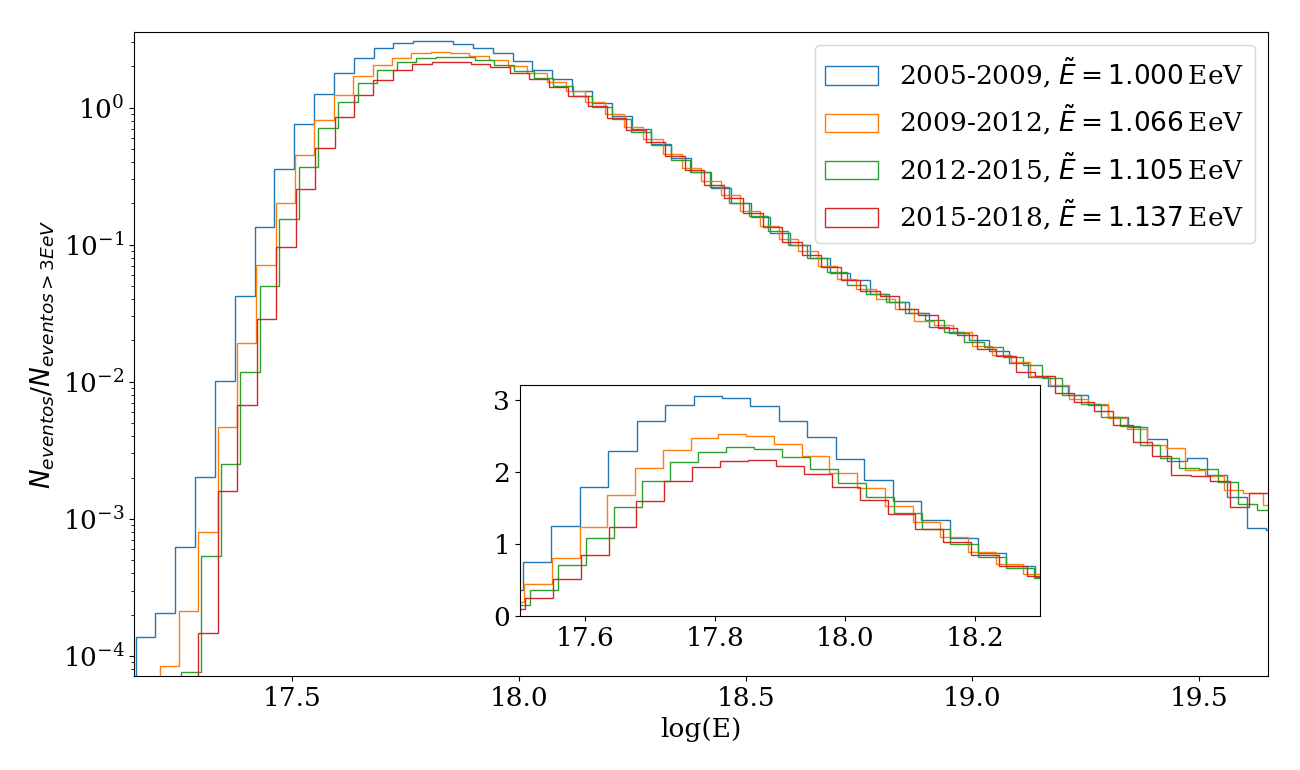
\includegraphics[width=0.8\textwidth]{histograma_evolucion_eventos.png}
	\caption{Histograma de eventos por rango de tiempo medido por el Observatorio Pierre Auger}
	\label{fig:futuro}
\end{figure}


El análisis del trabajo de licenciatura fue realizado sobre los eventos medidos utilizando el disparo estándar del arreglo principal, cuya eficiencia varía con la energía del CR. Para el disparo estándar, los eventos con energía mayor a $3\,$EeV y $\theta_{max}<60^o$ o  por encima de $4\,$EeV y $\theta_{max}<80^o$, son detectados con una eficiencia del 100\%. Por lo tanto, el análisis de anisotropías en el rango de energía entre $1\,$EeV - $2\,$EeV, se requieren factores relacionados a la eficiencia del disparo en función de la energía. Estos factores son obtenidos de manera fenomenológica \cite{taborda}. 

Para superar esta dificultad y para poder recuperar la sensibilidad para bajas energías, a partir del año 2013  se implementó otros algoritmos de disparo en los SDs, llamados ToTd y MoPS \cite{pierre2013plans}. Estos algoritmos de disparo se mencionan en este trabajo como \textit{todos los disparos}. La implementación de los ToTd y MoPS fue llevada a cabo mediante una actualización de la electrónica de los SDs para bajar el umbral de disparo, en particular para las señales de la componente electromagnética de la EAS, mejorando la reconstrucción mediante la separación fotón/hadrón para bajas energías. Con esta mejora, la eficiencia completa se alcanza a partir de una energía mayor a $1\,$EeV. De tal manera que, al estudiar los eventos en el rango $1\,$EeV - $2\,$EeV,  no son necesarios los factores de eficiencia y sólo pueden afectar los cambios de la exposición del observatorio.


Una desventaja de todos los disparos sobre el disparo estándar, es que el último tiene una mayor cantidad de años medidos en el rango $1\,$EeV - $2\,$EeV, ya que se adquieren datos  desde el año 2004 con ese algoritmo. Esto es conveniente ya que mientras más años han sido medidos es más factible efectos espúreos se cancelen. En cambio, para todos los disparos, el análisis de anisotropía con todos los disparos solo es posible desde el año 2013. Entre inicios del 2004 y finales del 2019, el conjunto de eventos del disparo estándar tiene $6\,975\,194$ eventos sin clasificar. En cambio entre mediados del 2013 hasta fines del 2019, el archivo de eventos para todos los disparos tiene $13\,739\,351$ eventos. El menor tiempo se compensa con la eficiencia de todos los disparos.


\section{Acerca de los eventos} \label{filtro}

Se aplican cortes a los eventos para asegurar la eficiencia completa de los detectores. Estos cortes implican límites en ángulo cenital $\theta$ de los eventos, en la cantidad de vecinos al tanque de mayor señal, además de restringirse a eventos medidos en condiciones normales, es decir, cuando los sistemas de comunicación del Observatorio funciona sin inconvenientes. De esta manera, podemos prescindir de otros factores de corrección.

A partir de los registros de eventos del arreglo principal con todos los disparos, se consideran solamente los eventos que cumplan las siguientes características:

    \begin{enumerate}
      \item La calidad de la reconstrucción depende de la energía y del ángulo cenital $\theta$ del evento.  Para eventos por debajo de los $4\,$EeV, se consideran los eventos con $\theta < 60^o$, en cambio para eventos por encima de esta energía se consideran $\theta < 80^o$.
      \item Los datos del evento son recopilados sin inconvenientes. Este filtro se conoce como \emph{Bad period flag} o $ib$. Un valor de 1 indica un buen periodo.
      \item Buena reconstrucción de la lluvia atmosférica asociada al evento.
      \item La cantidad de vecinos alrededor del tanque con mayor señal sea de 6 tanques, es decir, que el tanque de mayor señal este en el interior de un hexágono de tanques activos. Estos eventos se conocen como \textit{eventos 6T5}.
    \end{enumerate}


\subsection{Acerca del registro de hexágonos}\label{hexagonos_rate}

La cantidad de los hexágonos activos sobre el observatorio está relacionado con el filtro de eventos $6T5$, que garantiza la calidad de la reconstrucción del evento. El observatorio lleva un registro de la cantidad de hexágonos activos cada 5 min, además de registrar las condiciones atmosféricas en distintas estaciones de clima sobre la superficie del observatorio. 


\section{Acerca de la tesis de licenciatura}

Durante la tesis de licenciatura se analizaron los efectos de las condiciones atmosféricas durante el desarrollo de las EAS.  Se analizaron los datos adquiridos durante en el periodo 2005-2018 por el arreglo principal. De esta manera, se extendió los periodos estudiados anteriormente en los siguientes trabajos \cite{abraham2009atmospheric}, \cite{abreu2012description}   y \cite{aab2017impact}. 

Los efectos atmosféricos afectan principalmente a la atenuación  longitudinal y lateral de la componente electromagnética  de la EAS, en particular dependen fuertemente de la temperatura y presión. Estos efectos del clima sobre los eventos se caracterizan por parámetros dependientes de la presión, densidad y temperatura del momento de la detección del evento. Los mismos también dependen del ángulo cenital de los eventos y se utilizan para corregir las señales registradas por los SDs. Las correcciones del clima utilizadas por la colaboración Pierre Auger fueron implementadas a partir del trabajo \cite{aab2017impact}. 

Durante el trabajo de la licenciatura se imitó el análisis de la modulación del clima sobre el periodo 2005-2015 de \cite{aab2017impact}, obteniéndose resultados compatibles. También se estudió la modulación del clima mediante el valor del $S_{38}$ sin la corrección propuesta por \cite{aab2017impact} aumentando el rango de tiempo analizado hasta el 2018. Se observó que los parámetros del clima obtenidos en este análisis sobre  $S_{38}$  son compatibles con los utilizados en la reconstrucción oficial. %Se realizó una corrección de los efectos atmosféricos a la energía con estos coeficientes, observándose que la modulación es despreciable para energías mayores a $3\,$EeV al igual que la reconstrucción oficial.


%Durante la tesis de licenciatura se analizaron las variaciones en los parámetros del clima. Los mismos son utilizados en la corrección de los eventos adquiridos por el observatorio Pierre Auger. Estas variaciones son causadas por las distintas condiciones atmosféricas durante el desarrollo de las EAS. Se analizaron los datos adquiridos durante en el periodo 2005-2018 por el arreglo de SDs espaciados 1500 m entre sí, conocido como \emph{arreglo principal}. De esta manera, se extendió los periodos estudiados anteriormente en los siguientes trabajos \cite{abraham2009atmospheric}, \cite{abreu2012description}   y \cite{aab2017impact}. 


%This signal is corrected for atmospheric effects [18] that would otherwise introduce systematic modulations to the rates as a function of time of day or season. This could result in spurious influences on the distribution in sidereal time (a time scale that is based on the Earth’s rate of rotation measured relative to the fixed stars rather than the Sun, corresponding to 366.25 cycles/year) and hence could be a source of systematic effects for the anisotropies inferred. The atmospheric effects arise from the dependences of the longitudinal and lateral attenuation of the electromagnetic component of air showers on atmospheric conditions, in particular temperature and pressure. If not corrected, these could cause a modulation of the rates of up to $\pm$ 1.7\% in solar time.


\chapter{Métodos}
\graphicspath{{1_Metodo/}}
% METODOS
La información sobre el origen de los RCs puede ser obtenida mediante el estudio de la distribución de las direcciones de arribo de los eventos. Las irregularidades sobre el flujo casi isotrópico de los RCs, en un rango de energía, pueden deberse a  zonas del espacio donde se producen más RCs que en otras, estas irregularidades se conocen como anisotropías. 

El análisis de anisotropías a grandes escalas angulares suele ser hecho sobre las irregularidades de la distribución de eventos en ascensión recta $\alpha$, ya que el arreglo principal tiene una exposición direccional en función de esta coordenada casi constante \cite{referencia_anis}.

\section{Cálculo de los coeficientes de Fourier para el análisis de anisotropía en ascensión recta}

Las anisotropías son variaciones pequeñas por lo que eliminar todo factor espurio en el análisis es importante. Para obtener la amplitud de la misma en ascensión recta, se estudia la frecuencia sidérea ($f_{sid}=366.25\,$ ciclos/año) \cite{taborda}. Los errores sistemáticos debido a la modulación de eventos por el clima u otros errores propios de la adquisición de datos, aparecen en la frecuencia solar  ($f_{sid}=365.25\,$ ciclos/año), por lo que se debe tener en consideración el análisis de esta frecuencia. La frecuencia anti-sidérea ($f_a=364.25\,$ ciclos/año) es una frecuencia que puede indicar efectos sistemáticos en la amplitud de la anisotropía en la frecuencia sidérea \cite{farley1954sidereal}. La mezcla entre modulaciones diarias y anuales induce bandas laterales ubicadas a $\pm1\,$ciclo/año con respecto a la solar \cite{taborda}. Por estos motivos se toman estas frecuencias  como referencia.

%(REDACTAR)La frecuencia sidérea, como ya se mencionó antes, es la frecuencia en la cual las anisotropías reales en la distribución en ascensión recta de los RCs deberían aparecer. La frecuencia solar es importante para chequear la existencia de efectos sistemáticos asociados a particularidades propias del experimento y/o de las condiciones atmosféricas. 

% La frecuencia anti-sidérea es una frecuencia arbitraria que se encuentra a la misma distancia (1 ciclo/año) de la solar que la frecuencia sidérea pero en el lado opuesto. La frecuencia anti-sidérea adquirió cierta relevancia por los trabajos de Farley y Storey [89] en los que se mostraba, para un modelo específico, que la mezcla de modulaciones.que la mezcla de modu-
% laciones con diferentes frecuencias genera bandas lateralesalrededor de la frecuencia natural de la señal. Por ejemplo, una variación del flujo de
% RCs que combina modulaciones anuales y diarias de la forma

% Dicho de otro modo, esta mezcla de frecuencias induce bandas laterales ubicadas a
% ± 1 ciclo/año. La frecuencia f sol + 1 es la sidérea y f sol − 1 es la anti-sidérea. Por esta
% razón, es útil chequear las amplitudes en anti-sidéreo porque dan una idea de efectos
% sistemáticos remanentes que podrían estar afectando también a la señal en tiempo
% sidéreo


  \subsection{Variaciones relativas de los hexágonos} \label{peso_hexagonos}

Para corregir las variaciones de la exposición del observatorio, podemos definir un peso  $w_i$ por cada evento $i$, que corrige la variación  $\Delta N_{cell}(\alpha^0)$ en función de la ascensión recta del cenit del observatorio $\alpha^0$ durante el rango de tiempo estudiado. Estas variaciones pueden deberse al crecimiento del arreglo a través de los años,  por caídas en la comunicación del observatorio con los SDs u otros motivos. 

El factor $\Delta N _{cell}(\alpha^0)$ tiene en cuenta que la exposición  direccional  el observatorio no es uniforme en tiempo sidéreo.  Se obtiene sumando el número de celdas durante el periodo de medición, en cada segmento de $\alpha^0$ y luego se normaliza con el valor medio de los segmentos. Este término afecta solamente el análisis de Fourier en ascensión recta.


%El factor $\Delta N _{cell}(\alpha^0)$ tiene en cuenta que la exposición  direccional  el observatorio no es uniforme en tiempo sidéreo.  Se obtiene sumando el número de celdas durante el periodo de medición, con eventos descartados con tiempo muerto debido a probables de alimentación o problemas de comunicación o adquisición.  El número total de celdas en cada segmento de $\alpha^0$ es normalizada a valor medio. Este término afecta solamente el análisis de Fourier en ascensión recta.

%Si este este efecto no es corregido, dan lugar a una aparente está dado por un error sistemático en la adquisición de datos y no por fluctuaciones sobre el flujo de CRs. (REDACTAR) Además esta variación puede modular el número de  eventos en función del tiempo y aparecer como una anisotropía.

%$\Delta N _{cell}(\alpha^0)$ , allows for the fact that the effective aperture of the observatory is not uniform in sidereal time. This factor corresponds to the relative number of detector cells, i.e. the active detectors surrounded by at least five other active detectors, present when the right ascension of the zenith of the observatory equals $\alpha^0$ within binning accuracy. 

%It is obtained by adding the number of cells over the whole period of observations, with dead times due to power failures or to communication or acquisition problems discarded. 

%The total number of cells within each $\alpha^0$ bin is normalized to the average value [22].$\Delta N _{cell}(\alpha^0)$ is plotted in Fig. S2 with a bin width of $1^o$ . This term affects only the Fourier analysis in right ascension,

    Para calcular estos pesos $w_i$, se sigue el algoritmo presentado a continuación:
     
      \begin{enumerate}
        \item Se establecen una frecuencia $f$  y un rango de tiempo a estudiar. Por ejemplo, se desea estudiar la frecuencia solar entre el 1 de Enero del 2014 a las 12:00:00 GMT y 2019 hasta el 1 de Enero del 2020 a las 12:00:00 GMT.

        \item Cada dato del registro de hexágonos, tomado en un momento $t$ durante el rango seleccionado, se clasifica según la cantidad de horas desde un momento de referencia $t_0$. Esta referencia $t_0$ es el 1 de Enero del 2005 a las 00:00:00 GMT, o  $21\,$hs del 31 de Diciembre del 2004, según la hora local de Malargüe.

        \item Podemos asociar una coordenada angular $h$ a $t$  y $f$  utilizando la siguiente expresión:
         \begin{equation}
          h = (t-t_0) \times \frac{360^o}{24\text{hs}} \times\frac{f}{f_{Solar}} + h_0
          \label{eq:h_horas} 
        \end{equation}
        El factor $\nicefrac{f}{f_{Solar}}$ sirve para hacer un cambio de escala temporal entre los periodos de distintas frecuencias. Se usa como referencia la $f_{Solar}$ dado que las horas (solares) se basan en esta frecuencia, y el valor de $h_0=31.4971^o$ representa la ascensión recta del cenit del observatorio en el momento utilizado como referencia.
        
        \item  Para simplificar el cálculo del peso de los hexágonos, se divide los $360^o$ de la ascensión recta en $L$ segmentos de $\nicefrac{360}{L} ^o$ cada uno. Para clasificar un dato se  toma  el valor $h$  y se calcula
        \begin{equation}
          h' = h\, mod \,360 %=  h - 360\Big \lfloor \frac{h}{360} \Big \rfloor
          \label{eq:h_primado}
        \end{equation}
        donde la función $mod$ representa la función módulo que devuelve un número real positivo. Con el valor de $h'$ del dato, se asigna el mismo al segmento $k$ que le corresponde, mediante la siguiente expresión
        \begin{equation}
          k = \bigg \lceil \frac{h'}{360}\times L \bigg \rceil
        \end{equation}
        donde $\lceil a \rceil$ representa la función techo \footnote{La función techo da como resultado el número entero más próximo por exceso}. Por ejemplo, si optamos por $L=24$ y un dato en particular resulta con  $h=395\,^o$, esto implica que $h'= 35^o$ y que $k=\lceil 2.333 \rceil=3$, por lo tanto, este registro corresponde al segmento en la $3^{a}$ posición.

        \item Una vez clasificados todos los datos del registro de hexágonos, se calcula la suma  $N_{hex, j}$ de los datos que cayeron un segmento $j$ dado. Para definir la variación relativa de hexágonos  $\Delta N_{cell,k}$ de un segmento $k$ en particular, necesitamos la media de hexágonos por segmento $ \langle N \rangle$  para normalizar las variaciones.
       \begin{align}
         \langle N \rangle &= \sum^{L}_{i=1} \frac{N_{cell, i}}{L}  \qquad
         \Delta N_{cell,k} = \frac{N_{cell, k}}{\langle N \rangle}  \label{epepe}
       \end{align}

      \end{enumerate}
 En la Fig.\ref{fig:pesos_referencia} se muestran las variaciones relativas de los hexágonos en función de la ascensión recta del cenit del observatorio para las frecuencias mencionadas. Este análisis fue realizado en el marco del trabajo \cite{referencia_pesos} con eventos del periodo 2004-2017. 



       En la Fig.\ref{fig:pesos_ejemplo} se observan los valores obtenidos de $\Delta N_{cell,k}$  con el código escrito para este trabajo, en función de la ascensión recta del cenit  para $L=288$ segmentos. Se analizó el conjunto de datos  utilizado para obtener los resultados la Fig.\ref{fig:pesos_referencia}, con el fin de validar dicho código. Los datos se analizaron desde el 1 de Enero del 2004 a las 00:00:00\,GMT  hasta el 1 de Enero del 2017 a las 00:00:00\,GMT. Se  observa que estos los resultados obtenidos son compatibles con la Fig.\ref{fig:pesos_referencia}
      
      \begin{figure}[H]
          \centering
              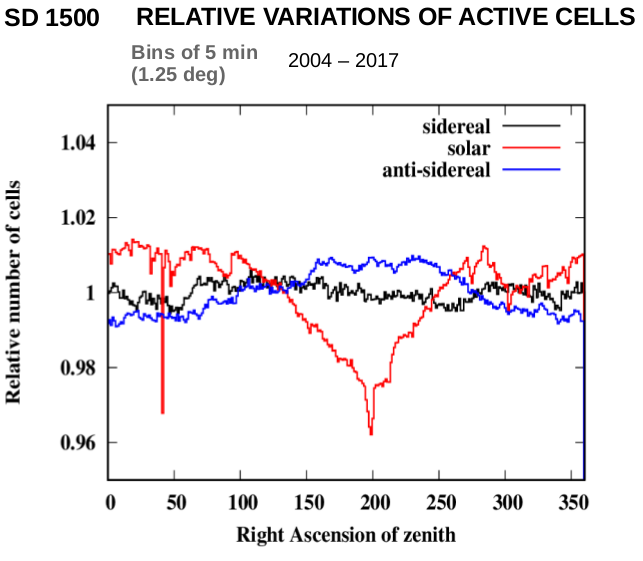
\includegraphics[width=0.5\linewidth]{pesos_referencia.png}  
              \caption{Valores de $\Delta N_{cell, k}$ en el rango 2004-2017 para distintas frecuencias obtenidas en el trabajo \cite{referencia_pesos}.}
              \label{fig:pesos_referencia}
        \end{figure}

       \begin{figure}[H]
          \centering
              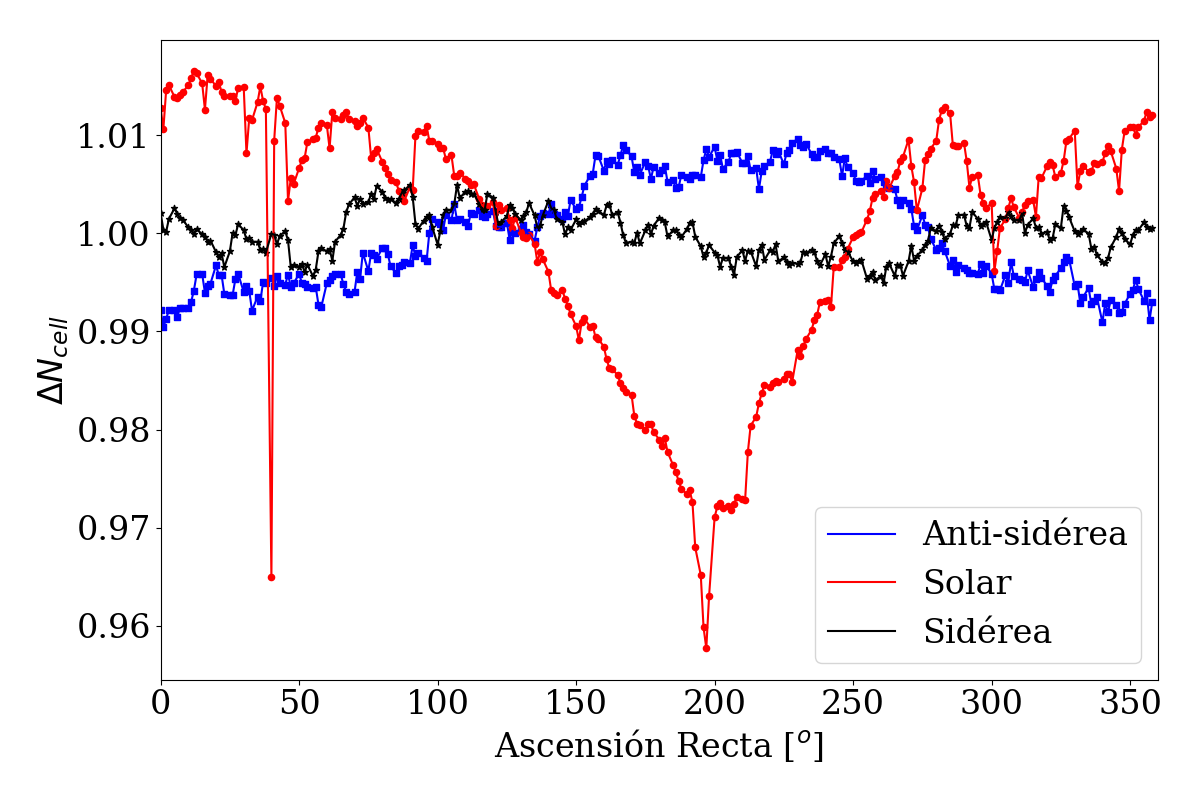
\includegraphics[width=0.75\linewidth]{weigths_2020.png}
              \caption{Valores de $\Delta N_{cell, k}$ en el rango 2004-2017 para distintas frecuencias utilizando el código escrito en este trabajo.}
              \label{fig:pesos_ejemplo}
        \end{figure}

     %Para la frecuencia solar, se observa una variación apreciable con respecto al $1$. Esto se debe a un problema en las

    Para una representación fiel entre los registros de los hexágonos y los pesos de los eventos, se optó por clasificar los datos de los hexágonos en $288$ segmentos, donde cada segmento tiene un ancho de $1.25^o$. Esto es conveniente ya que la actualización del registro de hexágonos se realiza una vez  cada $5\,$min como se menciona en la sección \ref{hexagonos_rate}. Esta tasa de actualización es equivalente a decir que la adquisición se realiza cada vez que el cenit del observatorio barre  $1.25^o$ en ascensión recta sobre la esfera celeste.


  \subsection{Cálculo de Rayleigh en ascensión recta para una frecuencia dada} \label{rayleigh}

%Rayleigh analysis in right ascension: A standard approach for studying the large-scale anisotropies in the arrival directions of cosmic rays is to perform a harmonic analysis in right ascension, $\alpha$. The first-harmonic Fourier components are given by 
  
  Un procedimiento para estudiar anisotropías en la direcciones de arribos de los RCs es realizar un análisis de Fourier en ascensión recta $\alpha$. La distribución en ascensión recta $\alpha$ del flujo de RCs $I(\alpha)$ que llega al arreglo principal puede caracterizarse por las amplitudes $r_k$ y fases $\phi_k$ de su expansión en serie de Fourier al $k-$ésimo orden. 

  \begin{equation}
    I(\alpha) = I_0 \bigg ( 1+ \sum^\infty_{k=1} r_k\cos{[k(\alpha - \phi_k)]} \bigg) = I_0 \bigg ( 1+ \sum^\infty_{k=1} a_k\cos{k\alpha} +  b_k\sin{k\alpha} \bigg ) 
  \end{equation}
  donde $a_k=r_k\cos\phi_k$ y $b_k=r_k\sin\phi_k$, y $I_0$ es el flujo medio. La distribución $I(\alpha)$ puede obtenerse a partir de la distribución de direcciones de arribo de los eventos observados.  En este trabajo, suponiendo que existieron $N$ eventos en el rango analizado, se considera que los mismos tienen una distribución en ascensión recta del tipo $\nicefrac{dN}{d\alpha}= \sum^N_{i=1} \delta(\alpha - \alpha_i)$ \cite{taborda}, de esta manera se simplifica el cálculo de $r_k$ y $\phi_k$. 

  Como se mencionó anteriormente, los análisis en ascensión recta están asociados a la frecuencia sidérea. Para realizar el análisis de los eventos en cualquier frecuencia arbitraria, es necesario modificar $\alpha$ por $\tilde{\alpha}$. Esta nueva variable tiene la forma como se utiliza en el trabajo \cite{taborda}:
  \begin{equation}
    \tilde{\alpha} = 2\pi f_x t_i + \alpha_i - \alpha_i^0(t_i) \label{ra_mod}
  \end{equation}
  donde $f_x$ es el frecuencia arbitraria a estudiar, $t_i$ es el momento en que ocurrió el evento y $\alpha_i^0(t_i)$ es la ascensión recta del cenit del observatorio en el momento del evento. Si la frecuencia a analizar es la sidérea, el análisis con $\alpha$ y $\tilde{\alpha}$ arrojan los mismos parámetros $r_k$ y $\phi_k$.

 Clasificando a los eventos mencionados en la sección \ref{specs} según el valor de la ascensión recta y considerando que todos los eventos tienen un peso uniforme de $w_i=1$, se dicen que los eventos fueron analizados \textit{sin pesos}, donde no consideramos la corrección de la exposición. En caso contrario, se habla de análisis \textit{con pesos} de los hexágonos  y estos pesos se calculan como se menciona en la sección anterior.

  Para realizar el análisis de frecuencias de los eventos, a primer orden en la expansión de Fourier, se siguen los siguientes pasos.

        \begin{enumerate}
        \item Fijando un rango de tiempo y un rango de energía en el cual se desea estudiar la anisotropía, se establece una frecuencia en particular $f$ a analizar. Siguiendo el ejemplo de la sección anterior, se analiza la frecuencia solar entre el 1 de Enero del 2014 a las 12:00:00 GMT y 2019 hasta el 1 de Enero del 2020 a las 12:00:00 GMT.

        \item Con los eventos ya filtrados según el criterio de la sección \ref{filtro}, asigno cada evento $i$ un valor $h_i$, definida en la Ec.\ref{eq:h_horas}

        \item En caso de considerar los pesos de los hexágonos, para asignar el peso correspondiente al evento, se asocia a un segmento $k$, calculado en la sección \ref{peso_hexagonos}, mediante el valor de $h'_i$ definido en la Ec.\,\ref{eq:h_primado}. Luego, el peso asignado $w_i$  al evento $i$ es: $ w_{i}= (\Delta N_{cell,k})^{-1}$, caso contrario, se toman que todos los eventos tiene $w_i=1$.
        
        \item Para el análisis en frecuencias, a partir del valor de $h_i$ se asigna el ángulo $\tilde{\alpha}_i$ definida en la Ec.\ref{ra_mod}. La implementación en el código es de la siguiente manera: 
        \begin{equation}
         \tilde{\alpha}_i = 2\pi \frac{h}{24} + \alpha_i -\alpha_{cenit,i}
        \end{equation}
        donde $\alpha_i$  representa la ascensión recta del evento y $\alpha_{cenit,i}$ la ascensión recta en el cenit del observatorio en el momento del evento. Cabe resaltar que la información de la frecuencia que se está estudiando, se encuentra en el cálculo de $h$. Si la frecuencia a estudiar fuera la sidérea, el término $2\pi \frac{h}{24} $ seguiría el cenit del observatorio, por lo que este término sería equivalente a $\alpha_{cenit,i}$, por lo tanto en esta frecuencia $ \tilde{\alpha}_i =\alpha_i$. %A partir de este ángulo $\tilde{\alpha}_i$ se realiza en análisis en frecuencias.

        \item Para calcular los coeficientes de Fourier del primer armónico $a$ y $b$, se siguen los siguiente pasos:
        \begin{enumerate}
          \item Por cada evento  $i$ se calculan los siguientes valores:
          \begin{align}
             a_i' = {w_i}\cos\tilde{\alpha}_i \qquad
             b_i' = {w_i}\sin\tilde{\alpha}_i
         \end{align}
         \item Una vez que se obtuvieron los valores de $a_i'$ y $b_i'$ para todos los eventos en el rango de tiempo estudiado, se calculan los coeficientes definidos en el trabajo \cite{analisis_fourier} mediante:
         \begin{alignat}{3}
          \mathcal{N} &= \sum^{Eventos}_i w_i \qquad
            a = \frac{2}{\mathcal{N}} \sum^{Eventos}_i a_i' \qquad
            b = \frac{2}{\mathcal{N}} \sum^{Eventos}_i b_i'  
         \end{alignat}
        \end{enumerate}
        \item Con los coeficientes es posible calcular la amplitud de la frecuencia estudiada $\tilde{r}$ y la fase $\phi$. Otros parámetros calculados para el análisis son la probabilidad $P(\tilde{r})$  y $r_{99}$. 
        \begin{alignat}{3}
            \tilde{r} &= \sqrt{a^2 +b^2}                        \qquad &&   \phi&&= \arctan\frac{a}{b}\\
          P(\tilde{r})&= \exp(-\mathcal{N}\frac{\tilde{r}^2}{4})\qquad &&   r_{99}&&= \sqrt{\frac{-4\log(0.01)}{\mathcal{N}}}
        \end{alignat}
        Cabe resaltar que el $r_{99}$ depende solamente de los pesos de los eventos que se está estudiando. La interpretación  de este valor es cual es la probabilidad de tener una amplitud mayor como una fluctuación de una distribución isotrópica sea del $1$\%
        %., y el valor de amplitud $r_{99}$ para que dicha probabilidad sea del $1$\%.
      \end{enumerate}

    Una forma de validar el código para el análisis de anisotropía es comparar los resultados del código con los obtenidos en otros trabajos \cite{taborda}. En la Fig.\ref{fig:sin_pesos_referencia} se muestra el análisis hecho sobre el mismo conjunto de eventos. Estos eventos fueron adquiridos con el disparo estándar desde el 1 de Enero del 2004 a las 00:00:00 GMT  hasta el 1 de Enero del 2017 a las 00:00:00 GMT. Se consideraron los eventos por encima de $8\,$EeV que además cumplan las condiciones dadas en la sección \ref{filtro}.  En esta figura que los resultados obtenidos en \cite{taborda} y con el código utilizado por este trabajo son indistinguibles. 

      \begin{figure}[H]
        \centering
        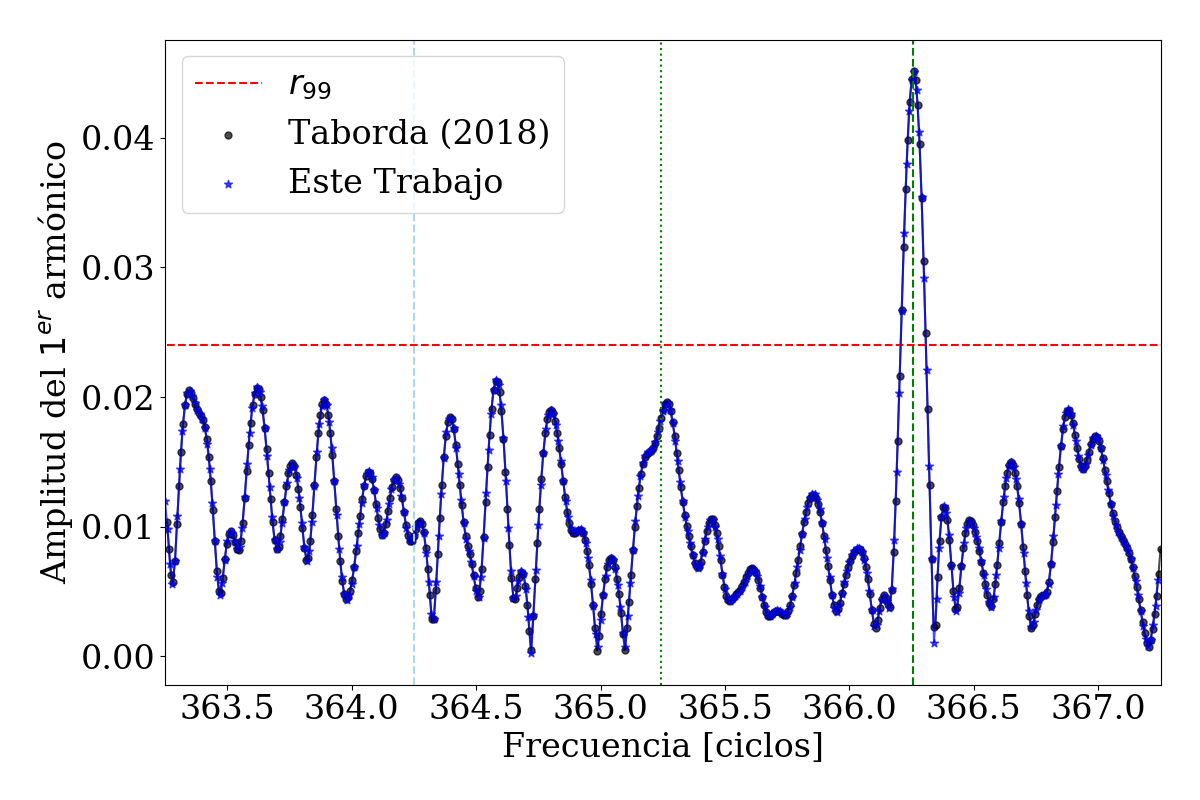
\includegraphics[width=0.75\linewidth]{sin_pesos_referencia_8_EeV.png}
        \caption{Comparación entre los análisis de anisotropía hechos para el mismo conjunto de datos, con el código de \cite{taborda} y con el código escrito para este trabajo.}
        \label{fig:sin_pesos_referencia}
      \end{figure}



% \chapter{Anisotropías en ascensión recta en los archivos con el disparo estándar}
% \graphicspath{{0_Introduccion/}}
% % RESULTADOS PARA ANISOTROPÍAS EN RA PARA LOS ICRC
  \section{Anisotropías en ascensión recta en los archivos del ICRC 2017 y ICRC 2019}

% ---> 8 EeV 
    \subsection{Eventos por encima de 8 EeV }

% ------> CARACTERISTICAS
     % \subsubsection{Características de los datos analizados}

% ------> ICRC 2017
      \subsubsection{Resultados para los datos del ICRC 2017}

      Para este apartado analicé el archivo de datos de la tesis de doctorado de Oscar Taborda, solamente los eventos 6T5. El rango de tiempo en el cual hice  el análisis es entre 1072969615 y 1472688000 ( 2004-01-01 15:06:55 y 2016-11-01 0:00:00 )

      Sabemos que para energía mayores de 8 EeV, aparece el dipolo en sidérea.

      En las Fig.\,\ref{fig:8EeV_sin_peso_ICRC2017_raw} y \ref{fig:8EeV_sin_peso_ICRC2017_cor} se muestra la amplitud del primer armónico sin considerar el peso de los hexágonos. Está figura es compatible con la Fig. 5.7.b, página 90 de la tesis de Taborda.

        \begin{figure}[H]
        
          \begin{subfigure}[b]{\textwidth}
          \centering
            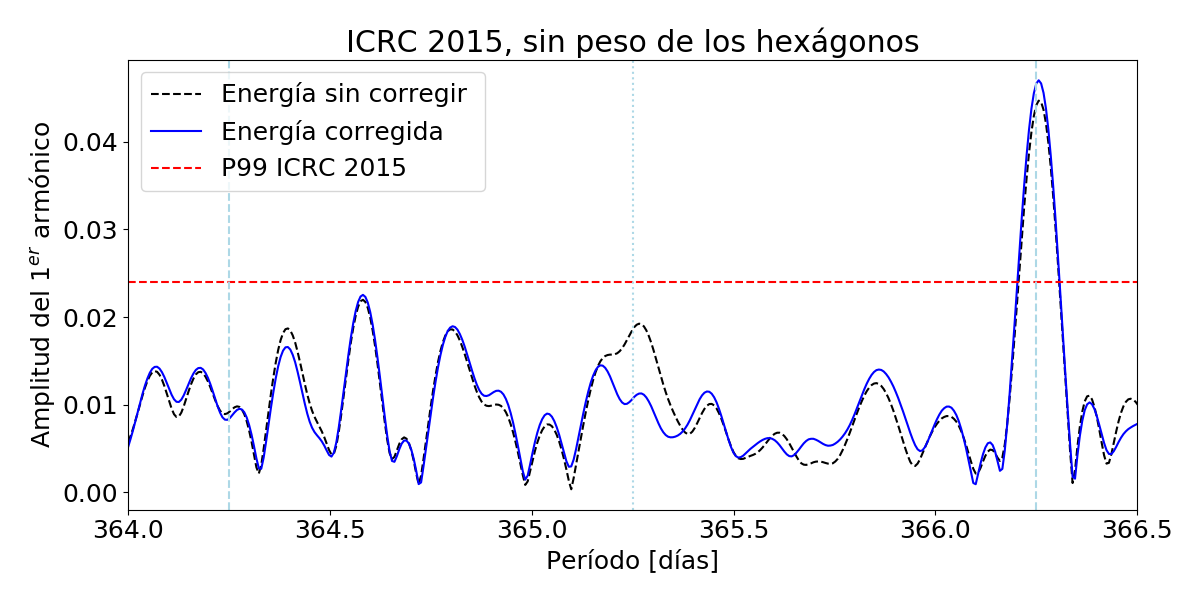
\includegraphics[width=\textwidth]{../0_Introduccion/ICRC/ICRC2017_Ecor_Eraw.png}
            \caption{Sin peso de la cantidad de tanques activos. }  \label{fig:8EeV_sin_peso_ICRC2017_raw}
          \end{subfigure}%
        
          \begin{subfigure}[b]{\textwidth}
          \centering
            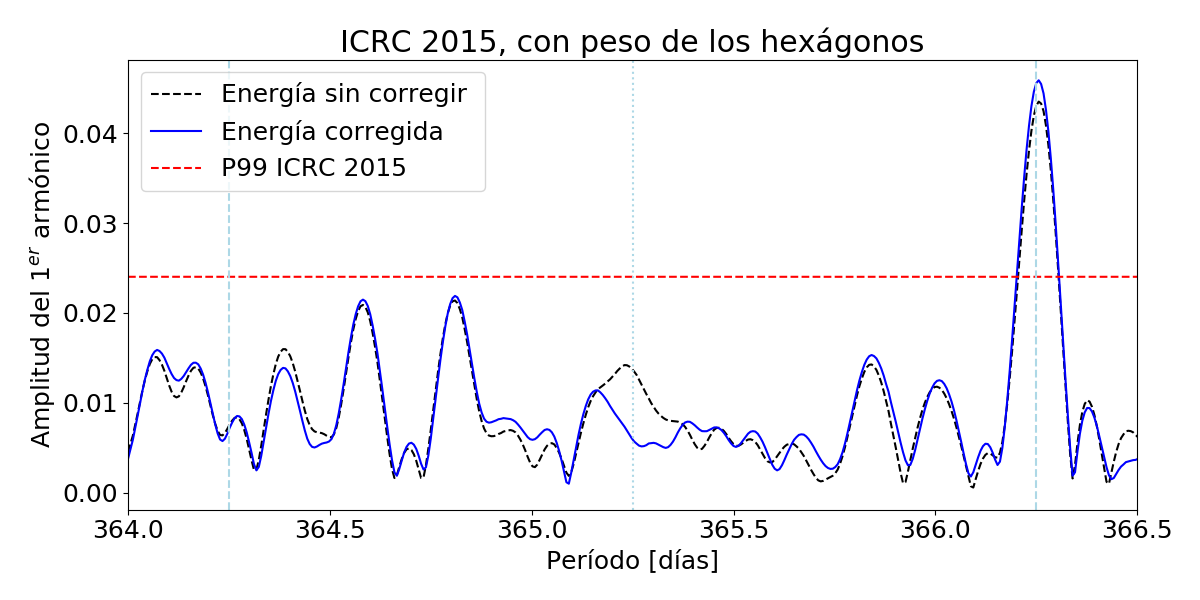
\includegraphics[width=\textwidth]{../0_Introduccion/ICRC/ICRC2017_Ecor_Eraw_hex.png}
            \caption{Con peso de la cantidad de tanques activos. }  \label{fig:8EeV_sin_peso_ICRC2017_cor}
          \end{subfigure}
          \caption{Primer armónico en ascensión recta de los datos del ICRC 2017}
        \end{figure}

      Con esto podemos decir que el código para la anisotropía funciona para el caso donde no se considera los hexágonos. No tengo un referencia para comparar las anisotropías con el peso de los hexágonos, solamente el valor del pico del dipolo.

% ------> ICRC 2019
      \subsubsection{Resultados para los datos del ICRC 2019}
      
      Este es el conjunto de archivos donde se hicieron modificaciones como el uso de una nueva reconstrucción y la corrección del clima. Usé solamente los eventos 6T5. El rango de tiempo en el cual hice  el análisis es entre 1072969615 y 1535789456 ( 2004-01-01 15:06:55 y   2018-09-01 08:10:56)

      \begin{figure}[H]
        \centering
        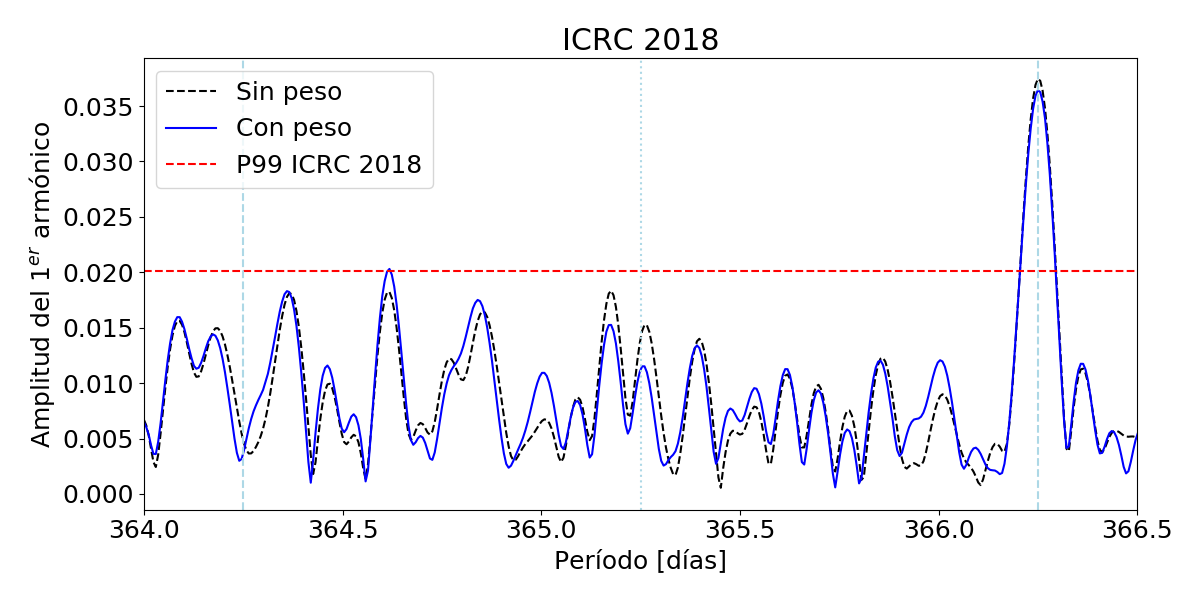
\includegraphics[width=\textwidth]{../0_Introduccion/ICRC/ICRC2019_Eraw_Eraw_hex.png}
        \caption{Primer armónico en ascensión recta de los datos del ICRC 2019.} \label{fig:8EeV_con_peso_ICRC2019}
      \end{figure}


      
% RESULTADOS PARA ANISOTROPÍAS EN RA PARA ALL TRIGGERS
  \section{Anisotropías en ascensión recta en los archivos con todos los disparos}
% ---> CARACTERISTICAS
    \subsection{Características de los archivos de datos analizados}

      Tenemos que tener en cuenta el archivo de datos de todos los disparos es entre los años 2013 y 2019, por lo que no podemos comparar los análisis de anisotropía con el conjunto  de datos del ICRC 2019 completo. Por lo que para compararlos, voy a hacer el análisis de ambos conjuntos de datos en el mismo rango de tiempo. Voy a hacer esto para poder comparar lo que sale.       Este rango donde se está comparando entre archivo empieza en  $utc_i = 1372699409 $.

    %CARACTERISTICAS GENERALES DE AMBOS SET DE DATOS.

      A continuación se presentan las características de los archivos estudiados, sin ningún filtro de energía, sin acotar por tiempo. 

      \begin{table}[H]
      \centering
        \begin{tabular}{c|c|c|c}
        \textbf{Archivo} & \text{Eventos} & UTC inicial &  UTC final  \\ \hline
        2020       & 13 739 351   &  1372680068 &  1577879983 \\
        2019       &  8 463 063   &  1372680068 &  1496318388 \\
        2017       &  8 592 302   &  1372680068 &  1498521517 \\
          \end{tabular}
      \end{table}
      
      Puede verse que el Archivo de 2020 tiene más eventos, y además de tener un rango de tiempo mayor que el archivo del 2017 y 2019. Los archivos 2017 y 2019  tienen $7\,072\,964$ eventos coincidentes y los archivos 2017 y 2020 tienen $6\,902\,21$ A continuación se compara la diferencia de energía y la calibración entre estos eventos.

    %COMPARANDO DELTA E ENTRE LOS DOS ARCHIVOS
      En las  Figs.\,\ref{fig:deltaE} y \ref{fig:histograma} se muestra la diferencia entre el valor de energía entre eventos coincidentes entre los archivos 2017 y 2020. Puede apreciarse que la diferencia no esta centrada 0 y no aparenta tener una modulación del clima. Por lo tanto la diferencia se debe a una reconstrucción distinta de los eventos.

          \begin{figure}[H]
            \begin{subfigure}[b]{0.5\textwidth}
              \centering
              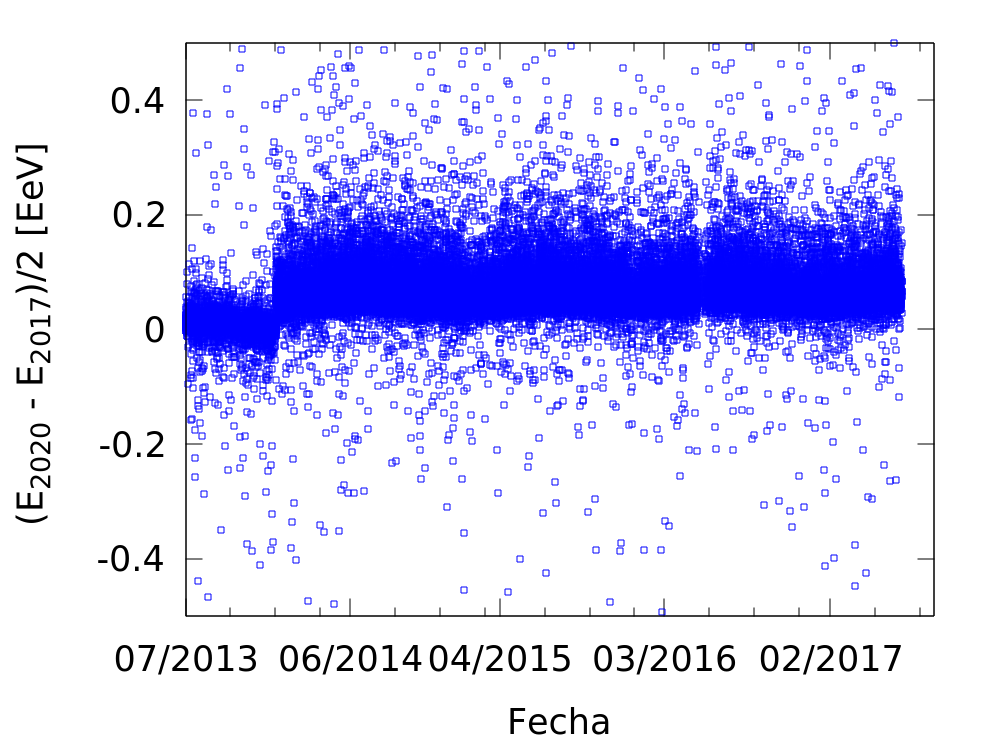
\includegraphics[width=\textwidth]{../0_Introduccion/comparacion_deltaE.png}
              \caption{Diferencia entre las energías} \label{fig:deltaE}
            \end{subfigure}%
            \begin{subfigure}[b]{0.5\textwidth}
              \centering
              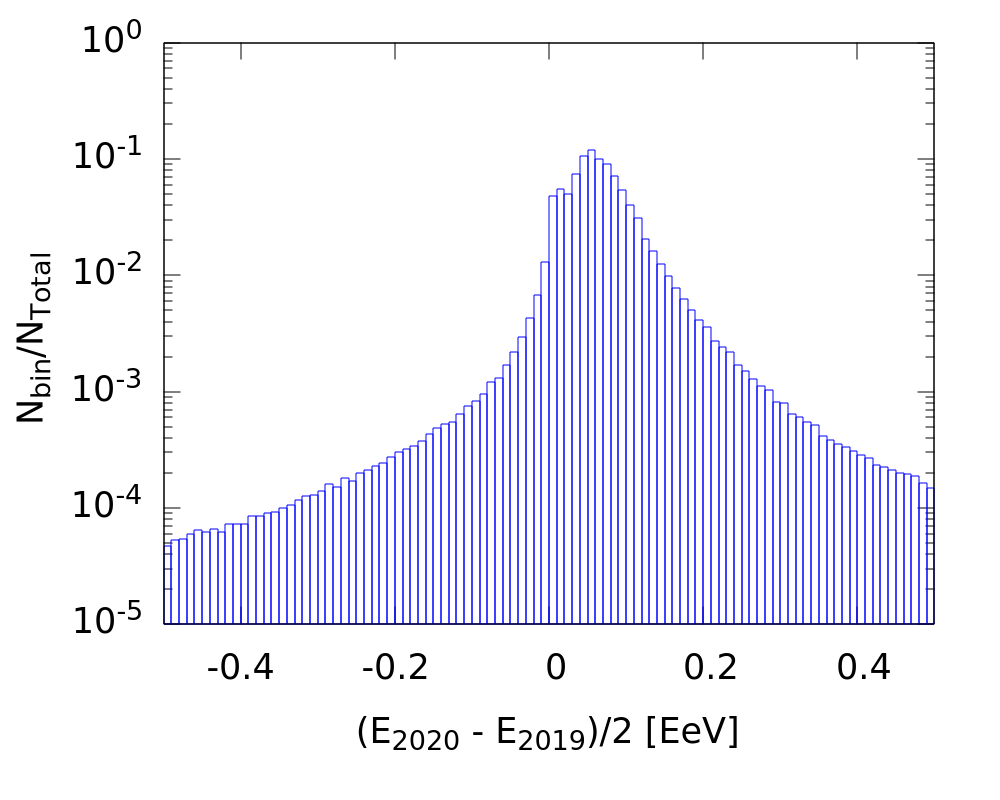
\includegraphics[width=0.8\textwidth]{../0_Introduccion/histograma_deltaE.png}
              \caption{Histograma de las diferencias}   \label{fig:histograma}
            \end{subfigure}
            \caption{Diferencia entre las energías del archivo de 2017 y el archivo del 2019}
          \end{figure}

    %COMPARANDO LA CURVA DE CALIBRACIÓN ENTRE LOS DOS ARCHIVOS
      Puede verse en la Fig.\,\ref{fig:calibracionE} que la curva de calibración entre ambos archivos es distinta, ya que la coordenada al origen como la pendiente es difieren entre para ambos archivos. Esto implica que los valores A y B de la curva $E=A\times (S_{38})^B$ son distintos para ambos conjunto de datos, ¿en qué afectaría? en primer lugar en el valor de la energía, segundo en análisis que dependan del estos parámetros como el análisis de la modulación del clima.

        \begin{figure}[H]
          \centering
          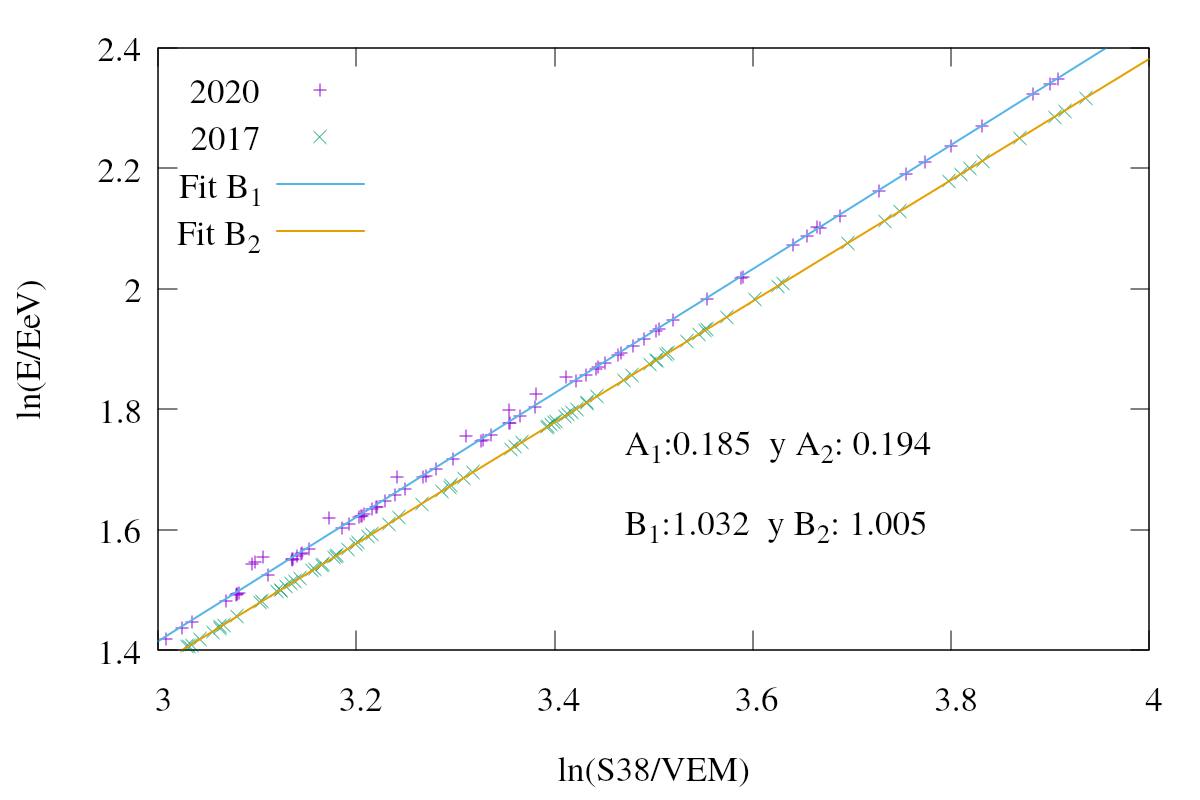
\includegraphics[width=0.65\textwidth]{../0_Introduccion/comparacion_reconstruccion.png}
          \caption{Calibración de las energías del archivo de 2017 y el archivo del 2019}
          \label{fig:calibracionE}
        \end{figure}



% \chapter{Report \#2: 27/04/2020 - Anisotropías para todos los disparos y pesos de los hexágonos}
% \graphicspath{{report_2_27_04_2020/}}
% 
\section{Anisotropías  considerando el peso de los hexágonos}

\subsubsection{Comparando los pesos en sidérea, solar y antisiderea.}


La idea que tengo sobre el pico en ambos gráficos es algo en la cantidad de hexagonos, algún periodo donde se apagó la mitad del observatorio o algo así.



\subsection{Variación de los pesos en función de la ascensión recta}
En las figuras de esta sección se muestran el análisis en ascensión recta para los eventos de observatorio considerando las variaciones de la exposición. 
Los mismos se hicieron en el mismo intervalo de tiempo para poder compararlos entre sí. Elegí el rango presentado en la Tabla \ref{rango_corto}  porque en el mismo se encuentran todos los eventos filtrados por energía, por bad period, por reconstrucción correcta, etc. El rango empieza en el 2013 porque la última versión del archivo de todos los disparos empezó a registrarse desde el  1 de Julio del 2013 a las 12:01:08 GMT (1372680068) hasta el  1 de enero del 2020 a las 11:59:43 (1577879983). Mientras que el archivo del disparo estándar va desde el 01 de enero del 2004.

	\begin{table}[H]
	\centering
		\begin{tabular}{c|c|c|c}
	 		& UTC 			& Fecha		 	&  Hora GMT  \\ \hline
	Inicio	& 1372699409	&2013-07-01 	&17:23:29		\\
	Final 	& 1577825634	&2019-12-31 	&20:53:54		\\
		\end{tabular}
	\caption{Rango de tiempo considerando todos los disparos} 	\label{rango_corto}
	\end{table}


\subsubsection{Energía entre 1\,EeV y 2\,EeV}

Para este caso utilizamos el archivo con todos los disparos en el rango de energía $1\,$ EeV - $2\,$EeV donde se tiene $1\,321\,702$ eventos.

\begin{figure}[H]
	\centering
	\includegraphics[width=0.5\textwidth]{Graficos/2019_AllTriggers_1_2_EeV_con_vs_sin_peso.png}
	\caption{Todos los disparos: entre 1 EeV y 2 EeV, entre 2013-2019}
	\label{fig:12w}
\end{figure}
%fig


La siguiente tabla se había calculado usando la formula 

\begin{equation}
	\tilde \alpha = 2\pi \frac{t_i}{T_x} +\alpha_i - \alpha^0
\end{equation}
donde $\alpha_i$ y $\alpha^o$ con las RA del evento y del cenit del observatorio.

	\begin{table}[H]
	\centering
		\begin{tabular}{c|c}
	 		&  2013-2019 (Con peso)	 \\ \hline
	Fase		& 	306.611				 \\
	$r$ 		&  0.00440897			\\
	$r_{99}$ 	&  0.00373348			\\
	$P(\tilde r)$ 	    & 	0.162485	\%	 \\
		\end{tabular}
	\caption{Rango de tiempo considerando todos los disparos} 	\label{rango_corto}
	\end{table}


\subsubsection{Energía entre 2\,EeV y 4\,EeV}

Para este caso utilizamos los eventos del archivo con todos los disparos con energía entre $2\,$ EeV - $4\,$EeV, donde se encontraron $288\,444$ eventos.
\begin{figure}[H]
	\centering
	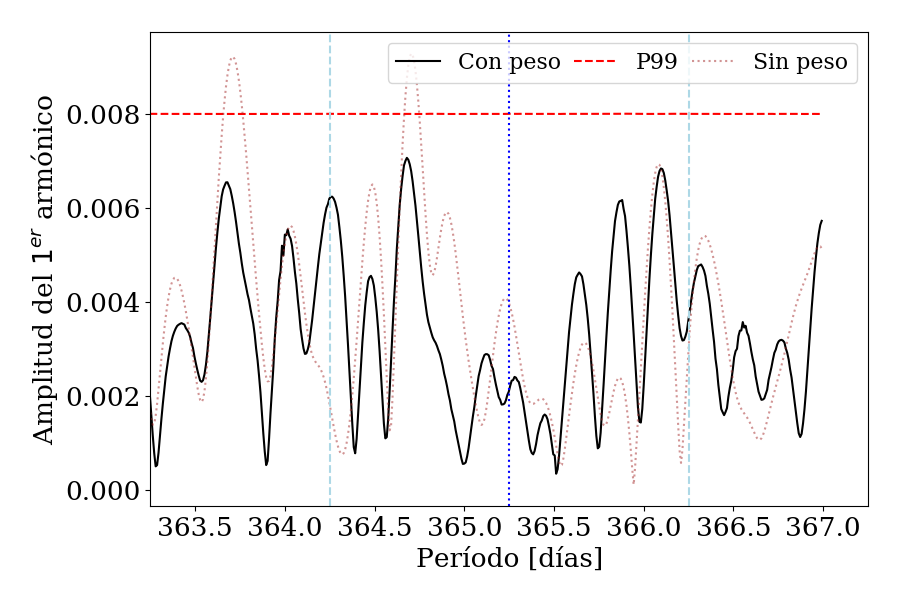
\includegraphics[width=0.5\textwidth]{Graficos/2019_AllTriggers_2_4_EeV_con_vs_sin_peso.png}
	\caption{Todos los disparos: entre 2 EeV y 4 EeV, entre 2013-2019}
	\label{fig:24w}
\end{figure}

En la Fig.\,\ref{fig:24w} no se ve ningún pico por encima de  percentil 99.


\subsubsection{Energía entre 4\,EeV y 8\,EeV}

A partir de $3\,$EeV el disparo estándar tiene una eficiencia del $100\%$. Entonces para este  intervalo de energías,  utilizamos el archivo con el disparo estandar.

\begin{figure}[H]
	\centering
	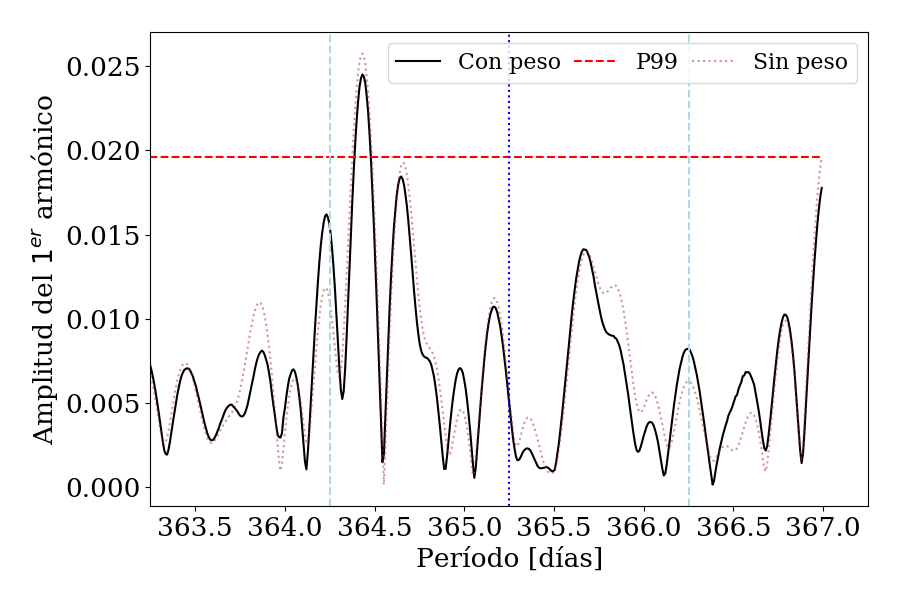
\includegraphics[width=0.5\textwidth]{Graficos/2019_Main_Array_4_8_EeV_con_vs_sin_peso.png}
	\caption{Disparos estándar: entre 4 EeV y 8 EeV, entre 2013-2019}
	\label{fig:48w}
\end{figure}
%fig

\subsubsection{Energía sobre 8\,EeV}

Para este caso utilizamos el archivo con el disparo estandar

\begin{figure}[H]
	\centering
	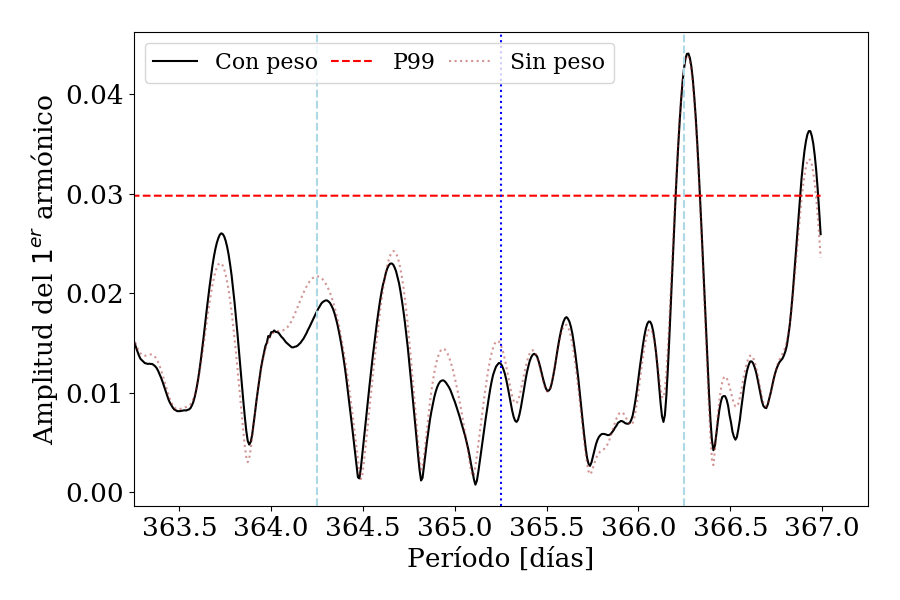
\includegraphics[width=0.5\textwidth]{Graficos/2019_Main_Array_8_EeV_con_vs_sin_peso.png}
	\caption{Disparos estándar: encima de 8 EeV, entre 2013-2019}
	\label{fig:8w}
\end{figure}
%fig




\subsection{Ampliando el rango de tiempo para el archivo del disparo estándar}

Amplié el rango de tiempo para poder compararlo con los gráficos anteriores, ya que se espera que mientras mayor sea el rango de tiempo los efectos espúreos disminuyen.

	\begin{table}[H]
	\centering
		\begin{tabular}{c|c|c|c}
	 		& UTC 			& Fecha		 	&  Hora GMT  \\ \hline
	Inicio	& 1104537600	&2005-01-01 	&00:00:00		\\
	Final 	& 1577825634	&2019-12-31 	&20:53:54		\\
		\end{tabular}
	\end{table}


\subsubsection{Energía entre 4\,EeV y 8\,EeV}

\begin{figure}[H]
	\centering
	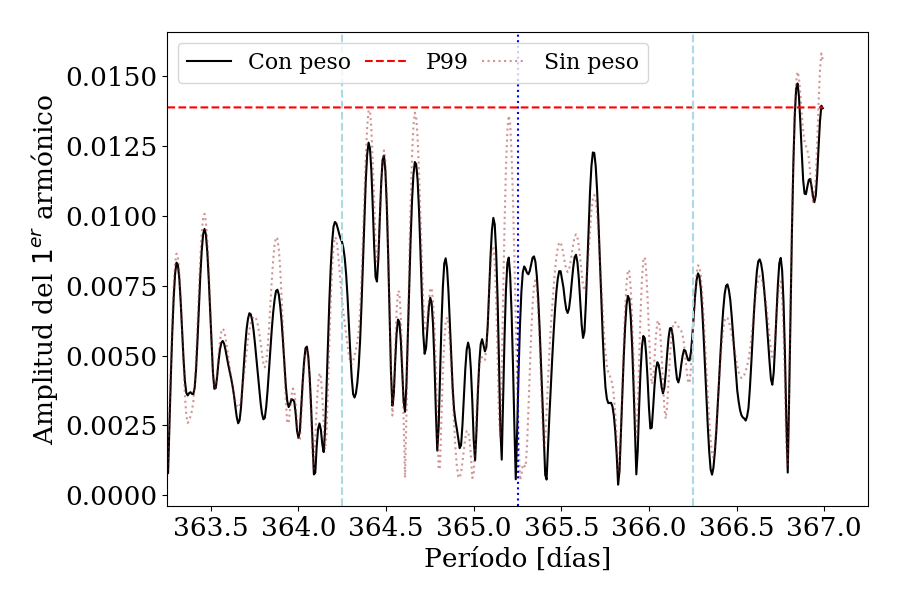
\includegraphics[width=0.5\textwidth]{Graficos/2019_Main_Array_4_8_EeV_con_vs_sin_peso_extended.png}
	\caption{Disparos estándar: entre 4 EeV y 8 EeV extendiendo el rango hasta el 2005}
	\label{fig:48w_extended}
\end{figure}
%fig

\subsubsection{Energía sobre 8\,EeV}


\begin{figure}[H]
	\centering
	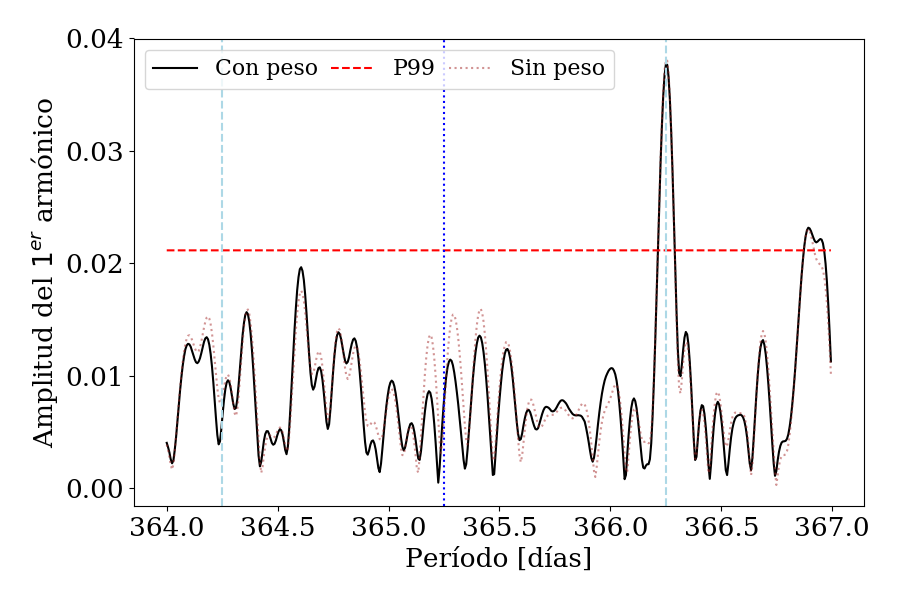
\includegraphics[width=0.5\textwidth]{Graficos/2019_Main_Array_8_EeV_con_vs_sin_peso_extended.png}
	\caption{Disparos estándar: encima de 8 EeV extendiendo el rango hasta el 2005}
	\label{fig:8w_extended}
\end{figure}
%fig

\chapter{Dipolo en el rango 1 EeV - 2 EeV}
\graphicspath{{6_Dipole_1-2_EeV/}}
\section{Características del conjunto de datos} \label{specs}

      Se debe tener cuenta que el archivo de evento para todos los disparos no es comparable con el conjunto  de datos del ICRC 2019. Porque el primero es entre los años 2013 y 2019 y el segundo se adquieren usando el disparo estándar.  Algo a considerar es que la colaboración cambió el algoritmo de reconstrucción de eventos en el 2019, con respecto al 2017.

    %COMPARANDO DELTA E ENTRE LOS DOS ARCHIVOS
      En las  Figs.\,\ref{fig:deltaE} y \ref{fig:histograma} se muestra la diferencia entre el valor de energía entre eventos coincidentes entre las reconstrucciones del año 2017 y 2020. Puede apreciarse que la diferencia no esta centrada 0 y no aparenta tener una modulación del clima. Por lo tanto la diferencia se debe a una reconstrucción distinta de los eventos.

    %COMPARANDO LA CURVA DE CALIBRACIÓN ENTRE LOS DOS ARCHIVOS
      Puede verse en la Fig.\,\ref{fig:calibracionE} que la curva de calibración entre ambos archivos es distinta, ya que la coordenada al origen como la pendiente es difieren entre para ambos archivos. Esto implica que los valores A y B de la curva $E=A\times (S_{38})^B$ son distintos para ambos conjunto de datos. Esto afectaría en primer lugar en el valor de la energía, y segundo a cualquier análisis que dependan de estos parámetros, como el análisis de la modulación del clima.

	Además de los filtros aplicados mencionados en la sección \ref{filtro}, se aplican filtros adicionales sobre la energía y el rango de tiempo. Para estudiar los eventos en esta sección, consideramos los eventos entre 1\,EeV y 2\,EeV de energía y que ocurrieron entre las 12:00:00 GMT del 1 de enero de 2014 y las 12:00:00 GMT del 1 de enero de 2020. Se centró en este rango de tiempo, ya que el registro de eventos más reciente al que se tuvo para hacer este trabajo termina el 1 de Enero del 2020  a las 11:59:43 GMT, además de para estudiar una cantidad entera de años, se optó por considerar los eventos desde el 1 de Enero del 2014 a las 12:00:00 GMT.

	Un resumen de todos los filtros aplicados se encuentra a continuación
		\begin{enumerate}
			\item Son eventos obtenidos mediante todos los disparos.
			\item Energía entre  [1 EeV , 2 EeV)
			\item Rango de tiempo:
			\begin{itemize}
				\item[-] Inicial:Jueves, 1 de Enero de 2014 12:00:00 GMT o 1388577600 UTC
				\item[-] Final:  Jueves, 1 de Enero de 2020 12:00:00 GMT o 1577880000 UTC
			\end{itemize}

		\end{enumerate}
	Aplicando estos filtros, se tienen $1\,081\,844$ eventos para estudiar en este rango de energía. 


        \begin{figure}[H]
          \centering
            \begin{subfigure}[b]{0.65\textwidth}
              \centering
              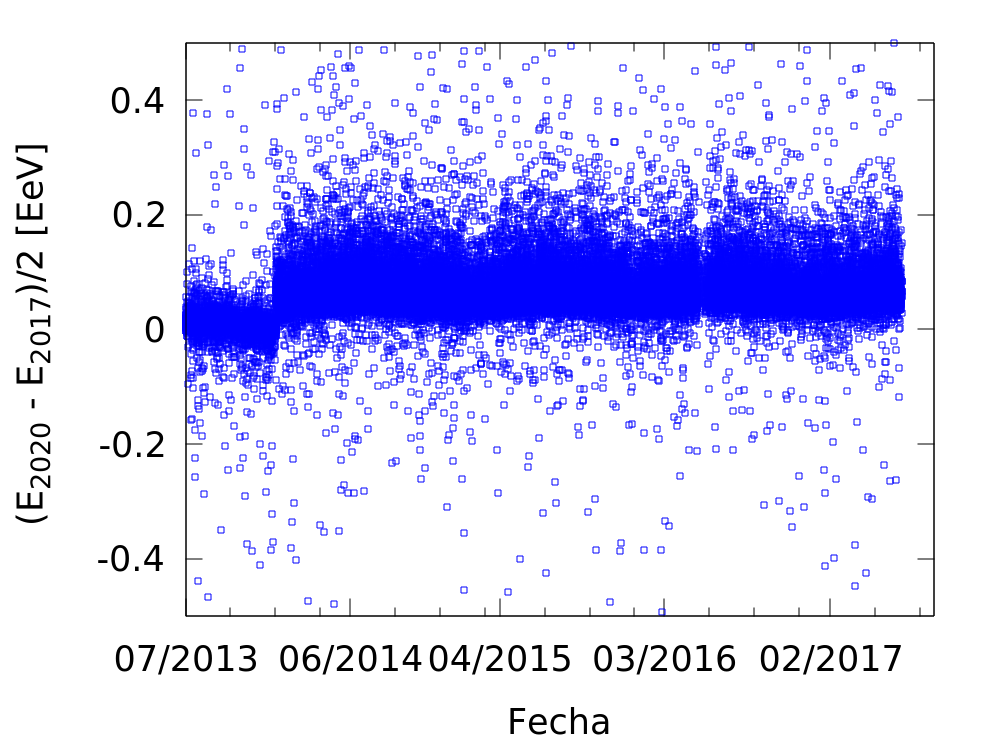
\includegraphics[width=\linewidth]{../0_Introduccion/comparacion_deltaE.png}
              \caption{Diferencia entre las energías} \label{fig:deltaE}
            \end{subfigure}\\
            \begin{subfigure}[b]{0.65\textwidth}
              \centering
              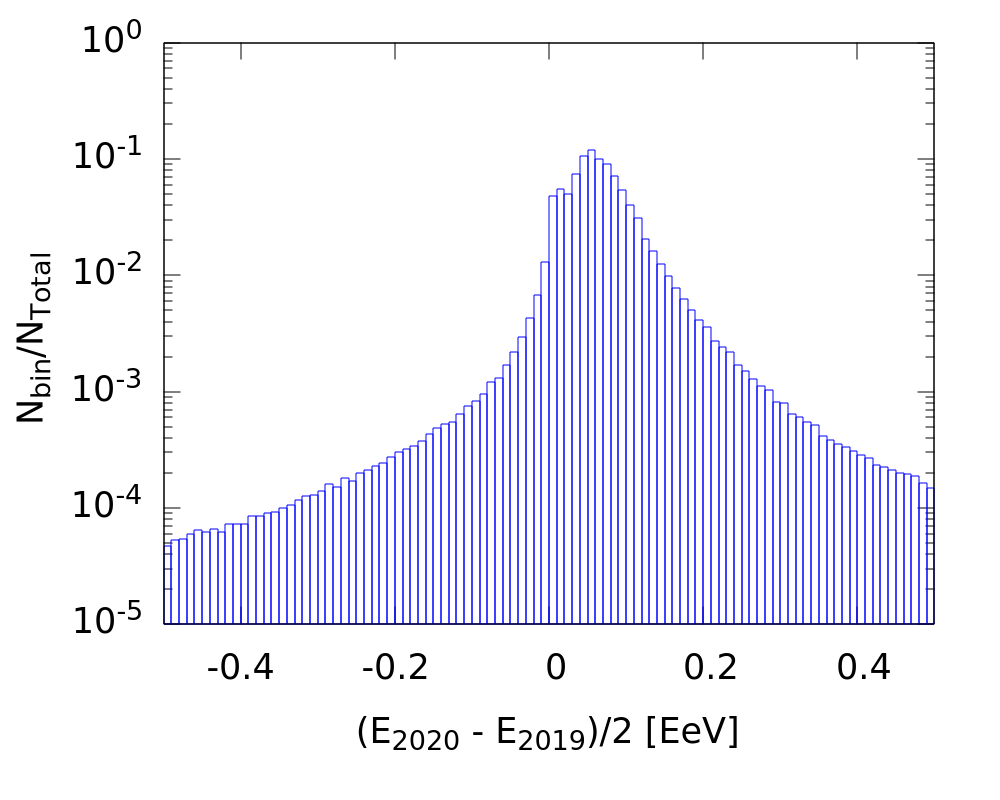
\includegraphics[width=\linewidth]{../0_Introduccion/histograma_deltaE.png}
              \caption{Histograma de las diferencias}   \label{fig:histograma}
            \end{subfigure}
           \caption{Diferencia entre las energías de entre la reconstrucción del 2017 y del 2019}
         \end{figure}

        \begin{figure}[H]
          \centering
          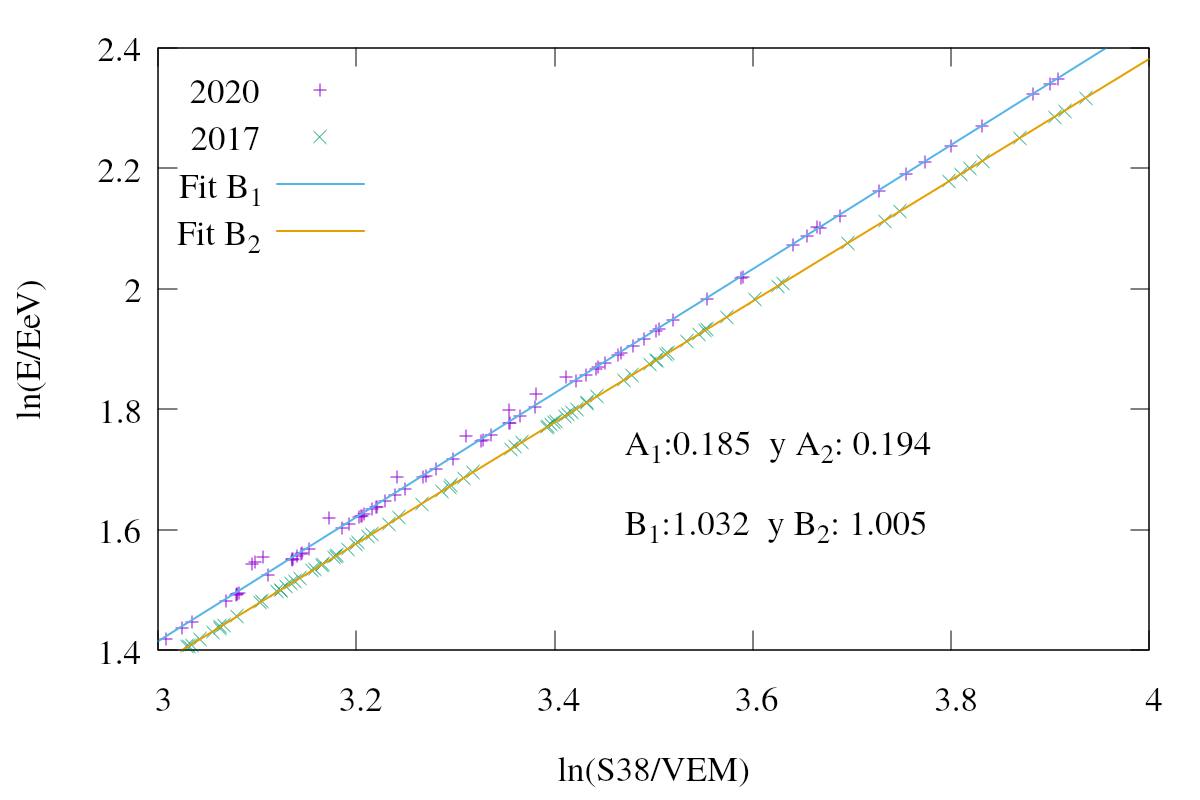
\includegraphics[width=0.65\textwidth]{../0_Introduccion/comparacion_reconstruccion.png}
          \caption{Calibración de las energías del archivo de 2017 y el archivo del 2019}
          \label{fig:calibracionE}
        \end{figure}
	
\section{Pesos de los eventos para frecuencias de referencia}

	 En la Fig.\,\ref{pesos_bin_1_2} se muestran los valores de  $\Delta N_{cell,k}$ en el rango donde se consideran los eventos. 
			 
			\begin{figure}[H]
				\centering
				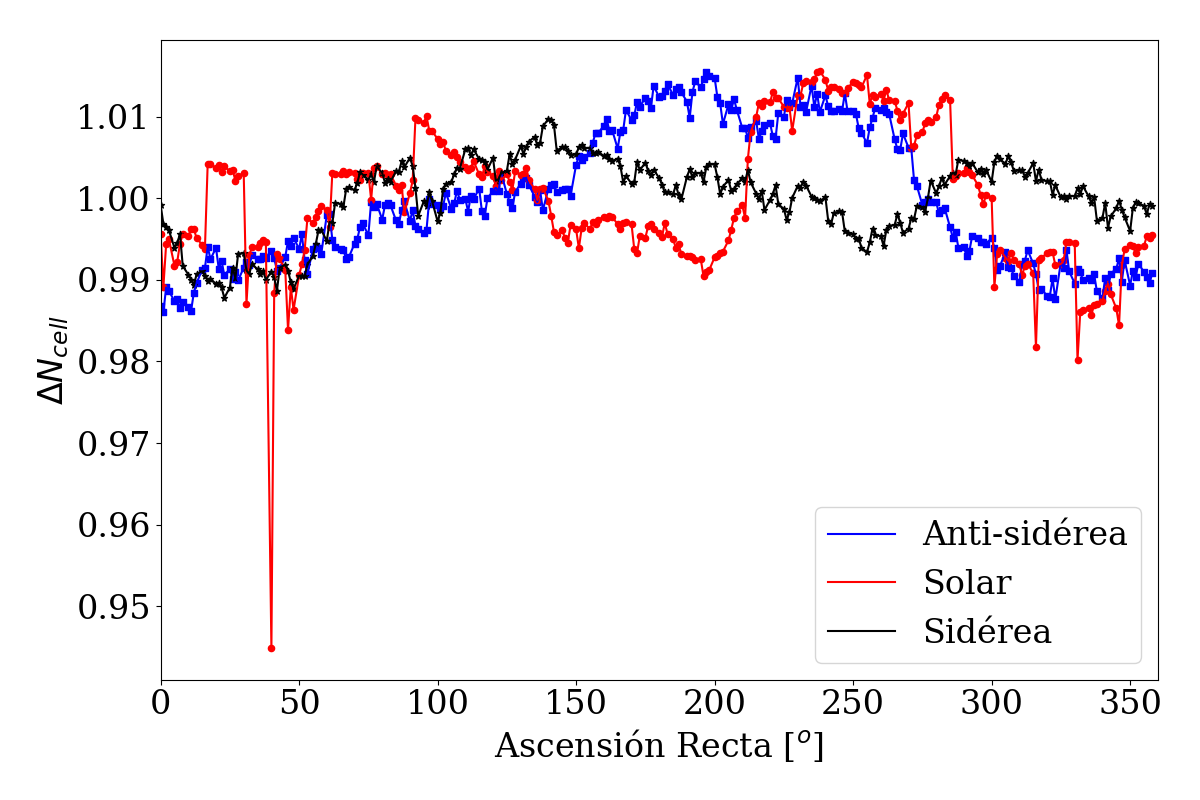
\includegraphics[width=0.75\textwidth]{weights_2013_2020.png}
				\caption{Variaciones de los hexágonos para frecuencias características en rango mencionado. }
				\label{pesos_bin_1_2}
			\end{figure}


	A cada una de estas frecuencias, se ajusta una función del tipo  $f(x)=a\cdot \cos{(\alpha-\phi)} + 1$, con el se busca aproximar la amplitud $a$ y el desfase $\phi$ de las curvas de los pesos en función de la ascensión recta $\alpha$. Los ajustes se observan en las Figs. \ref{fig:ajuste_antisiderea}, \ref{fig:ajuste_solar} y \ref{fig:ajuste_siderea}.


	\subsection{Gráficos de los ajustes}

Para verificar los valores de amplitud y fase en la frecuencia sidérea, se ajusta una función del tipo 
\begin{equation}
	f(RA) = a\cos{(2\pi(\omega RA + \phi))} +c
\end{equation}

a la variación de los hexágonos por ángulos de ascensión recta $RA$, así como también a la variación de los pesos de los eventos en ascensión recta \footnote{El peso de los eventos es la inversa del peso de los hexágonos}. En el ajuste, se dejan libres los parámetros de la amplitud $a$, desfase $\phi$ y offset $c$, en cambio la frecuencia $\omega=1$, ya que los valores de ascensión recta $0^o$ y $360^o$ son equivalentes y estamos trabajando con el primer armónico. La variación y el ajuste puede verse en las Figs.%\ref{fig:pesos_ajuste} y \ref{fig:pesos_hexagonos}.

Los valores de los ajustes, comparados con el análisis de Rayleigh se muestran en la Tabla\,\ref{tabla:ajuste_primer_armonico}. SE observa que el valor de la amplitud para el caso de la variación de los pesos es más cercana al que se obtuvo en el análisis de Rayleigh. Esto puede deberse que los pesos están normalizados por la integral de todos los hexágonos dada un frecuencia, por lo que si existe alguna constante multiplicativa en la cantidad de hexágonos, la amplitud la tabla para la primera columna puede no ser igual a la segunda columna.

\begin{table}[H]
\centering
\begin{tabular}{l|c|c|||c}
				& Hexágonos 				& Pesos	de los eventos		& Rayleigh con peso \\ \hline
%Figura:			& \ref{fig:pesos_hexagonos} &\ref{fig:pesos_ajuste}		&\ref{fig:zoom} \\
Fase $\phi$:	& 284.874 	 				& 285.099					&329.865	\\
Amplitud $a$:	& 0.00784107 				&  0.00384774 				&0.004676\\
\end{tabular}
\caption{Fase y amplitud del ajuste del primer armónico en ascensión recta en los hexágonos y  pesos  de los eventos para la frecuencia sidérea}
\label{tabla:ajuste_primer_armonico}
\end{table}


		
		\begin{figure}[H]
		\centering
		\begin{subfigure}{.75\textwidth}
			\centering
			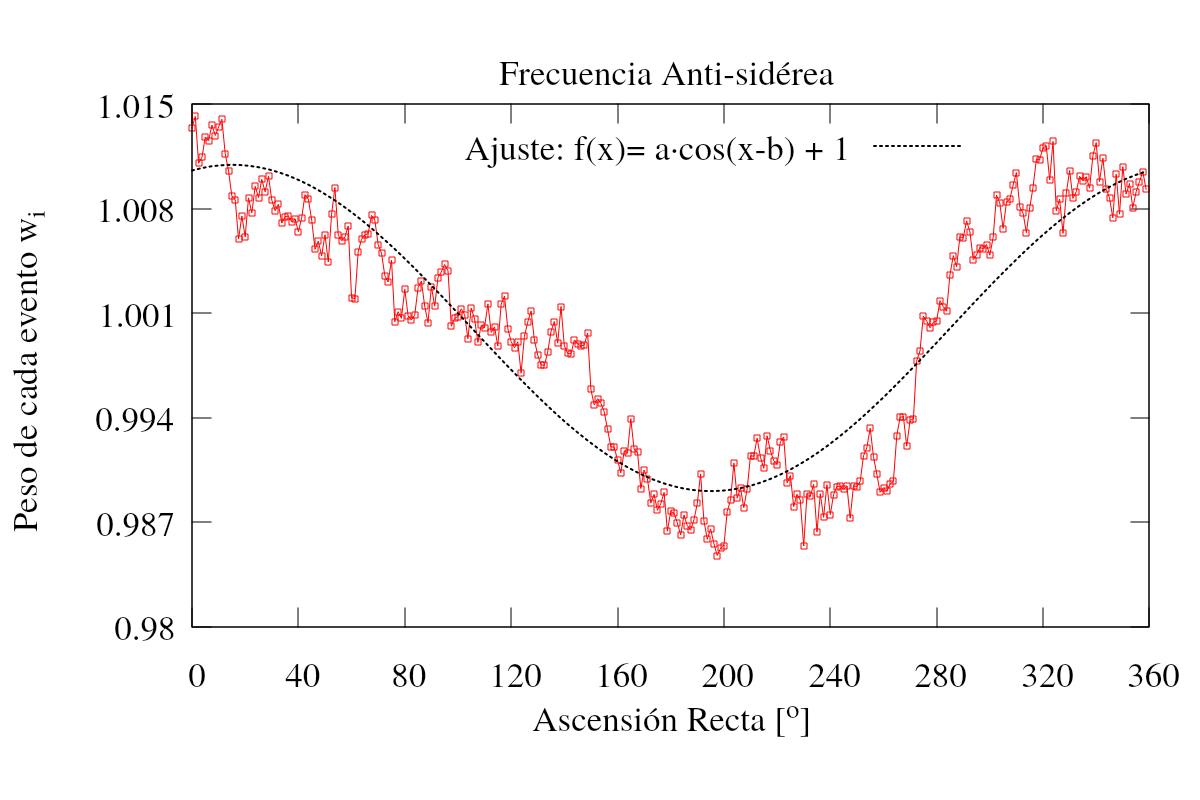
\includegraphics[width=\linewidth]{eventos_RA_ajuste_cos_antisiderea_v2.png}
			\caption{Frecuencia anti-sidérea}
			\label{fig:ajuste_antisiderea}
		\end{subfigure}\\
		\begin{subfigure}{.75\textwidth}
			\centering
			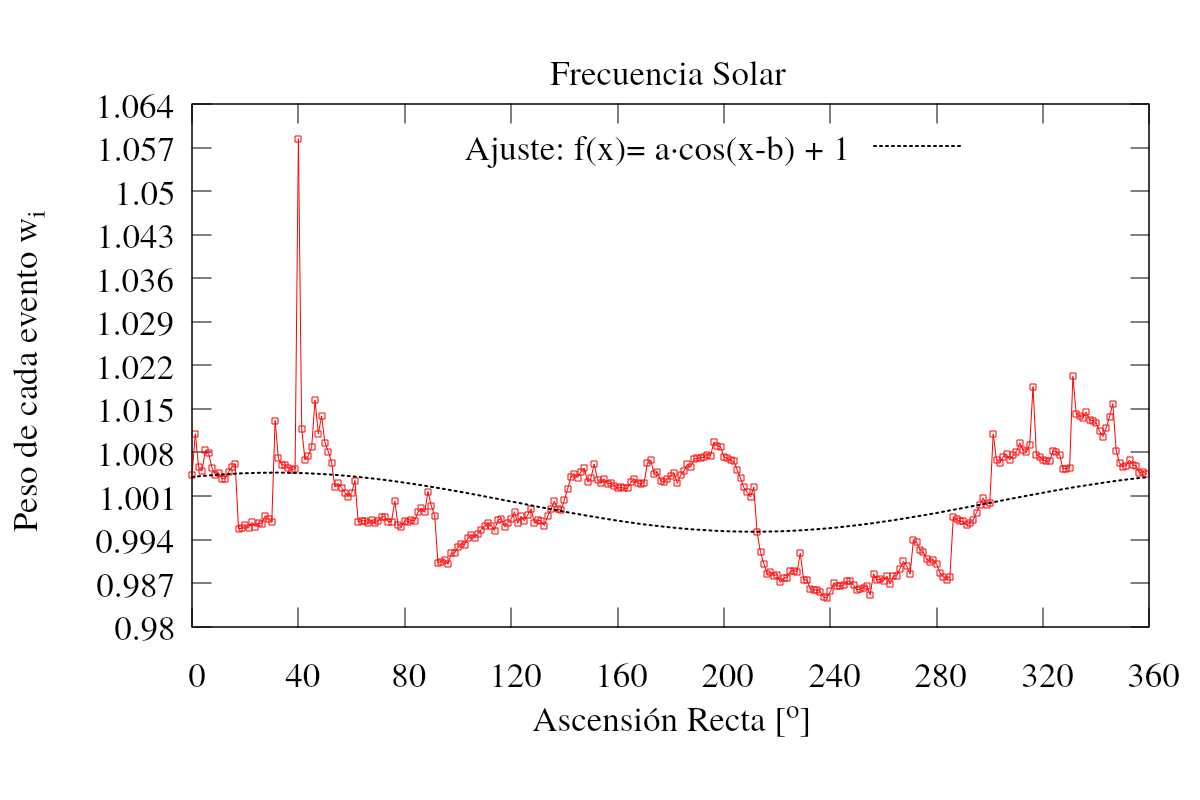
\includegraphics[width=\linewidth]{eventos_RA_ajuste_cos_solar_v3.png}
			\caption{Frecuencia solar}
			\label{fig:ajuste_solar}
		\end{subfigure}\\
		\centering
		\begin{subfigure}{.75\textwidth}
			\centering
			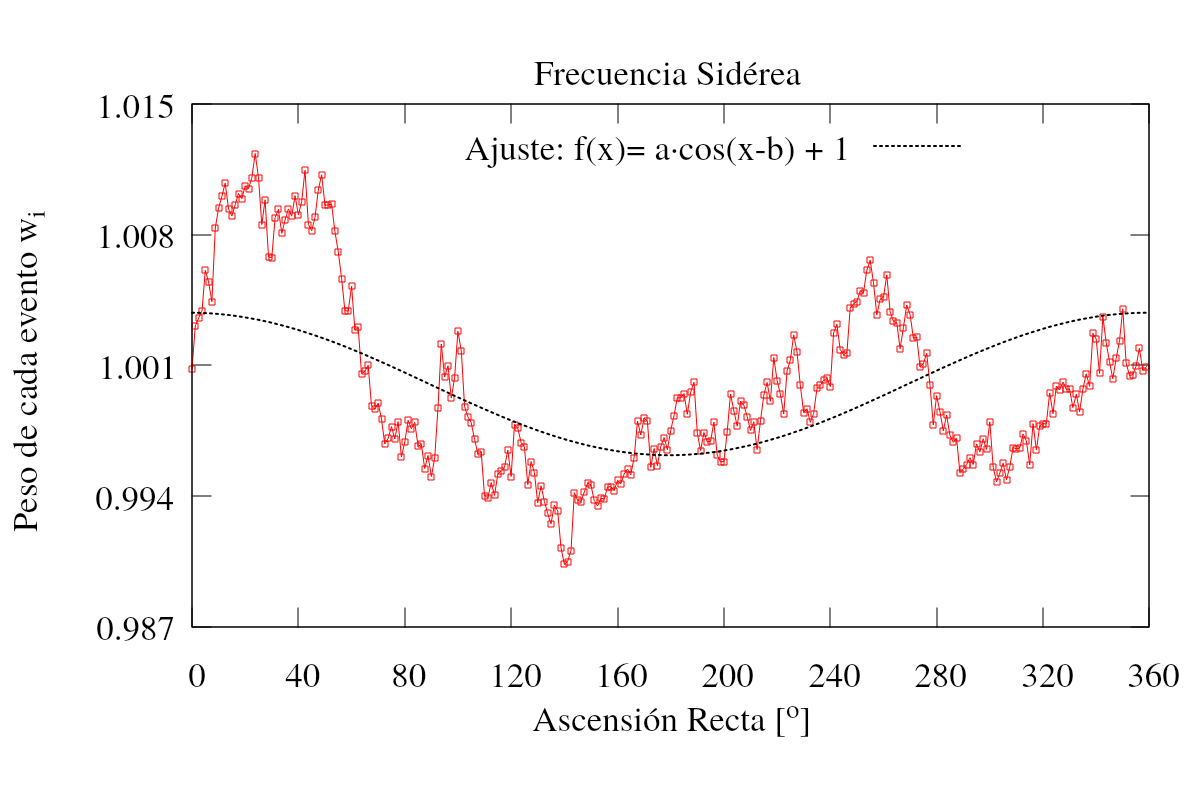
\includegraphics[width=\linewidth]{eventos_RA_ajuste_cos_siderea_v2.png}
			\caption{Frecuencia sidérea}
			\label{fig:ajuste_siderea}
		\end{subfigure}%
		\caption{Ajuste de los pesos de los eventos para varias frecuencias a primer orden en ascensión recta}
		\end{figure}
		
	
\subsection{Tabla comparando los ajustes:}
		
		\begin{table}[H]
		\centering
		\begin{tabular}{c|c|c|c}
					& Anti-sidérea			& Solar 				& Sidérea\\ \hline
		Amplitud $a$& $0.0109\pm 0.0003 $ 	&	$0.0038 \pm 0.0003$	&  $0.0047\pm 0.0007$		\\
		Fase $\phi$ & $15    \pm 1$ 		&   $360 \pm 5   $ 		&  $31    \pm 8    $ 		\\
		\end{tabular}
		\caption{Parámetros obtenidos del ajuste a primer orden en $\alpha$ sobre los pesos.}
		\end{table}


\section{Gráfico de la anisotropía}

 En las figuras de esta sección se muestran el análisis en ascensión recta para los eventos de observatorio considerando las variaciones de la exposición.

 Los mismos se hicieron en el mismo intervalo de tiempo para poder compararlos entre sí. 
 
%Elegí el rango presentado en la Tabla \ref{rango_corto}  porque en el mismo se encuentran todos los eventos filtrados por energía, por bad period, por reconstrucción correcta, etc.



% \begin{table}[H]
% \centering
% \begin{tabular}{l|c|c}
% 				& Con Peso 	& Sin peso 		\\ \hline
% Frecuencia:		& 366.25 	& 366.25 		\\
% Fase:			& 329.865 	& 292.312		\\
% $P(r)$:			& 0.76398\%	& 26.6838 \% 	\\
% Amplitud:		& 0.004676 	& 0.00243515	\\
% \end{tabular}
% \caption{Fase, $r_{99}$ y $P_{99}$ del análisis de anisotropía }
% \end{table}



%En la Fig.\ref{fig:zoom} se muestra el pico que se presenta en  el intervalo de energía entre 1 EeV - 2 EeV, cercano a la frecuencia sidérea. El pico tiene un máximo para un período de $366.21$. En la Tabla.\,\ref{tabla:pico} se muestran los valores de la fase, $r_{99}$ y $P_{99}$ para el periodo anterior.

% \begin{figure}[H]

	\subsubsection{Análisis de anisotropías en ascensión recta}
		
		\begin{figure}[H]
			\centering
			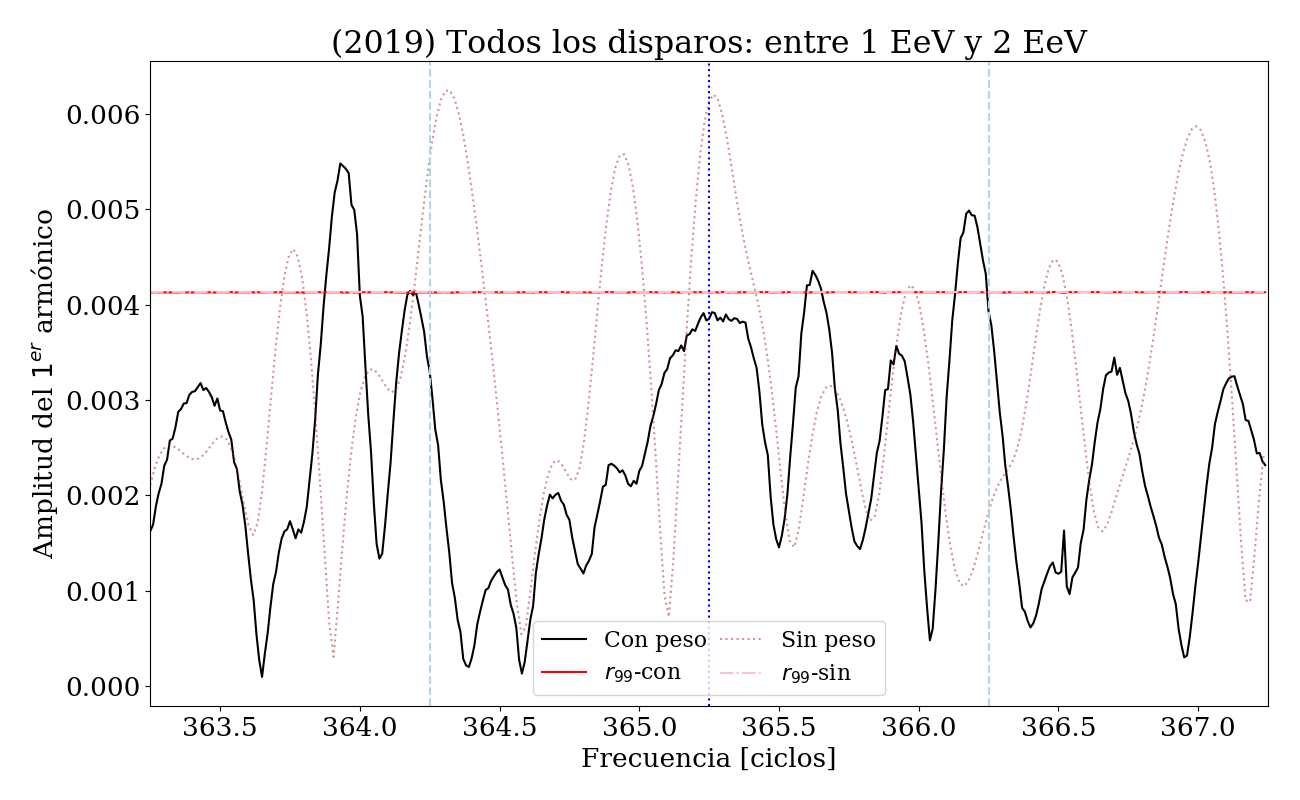
\includegraphics[width=0.75\linewidth]{pesos_sin_con_1_2_EeV.png}
			\caption{Anisotropía en función de la frecuencia, se comparan los análisis sin los pesos y con los pesos de los hexágonos}
		\end{figure}
		

		\begin{table}[H]
		\centering
		\begin{tabular}{l|l|l|l|l}
			\multicolumn{1}{c}{}  & \multicolumn{2}{c}{Sin pesos}  & \multicolumn{2}{|c}{Con pesos} \\ \hline
			Frecuencia:   & Solar         & Sidérea        & Solar         & Sidérea        \\ \hline
			Fase $\phi$:  & 251           & 289            & 288           & 335            \\ \hline
			Amplitud $r$: & 0.0061        & 0.0018         & 0.0038        & 0.0039         \\ \hline
			$P(r)$:	      & 0.004 \%	  & 41\%	   	   & 2 \%          & 1 \% 	\\
		\end{tabular}
		\caption{Comparación de los parámetros de fase y amplitud para las frecuencias sidérea y solar, analizando sin pesos y con los pesos de los hexágonos con el análisis de Rayleigh entre en 1 de Enero del 2014 y el 1 de Enero del 2020}
		\end{table}
		
		% \begin{table}[H]
		% \centering
		% \begin{tabular}{c|c|c|c|c|c}
		% Frecuencia	& Solar (sin peso)	& Solar (con peso)	&& Sidérea (sin peso) 	& Sidérea (con peso)	 \\ \hline
		% Fase $\phi$ & 251	    		& 288	    		&& 289				& 335				\\
		% Amplitud $r$& 0.0061	    	& 0.0038	  		&&0.0018		& 0.0039			\\
		% \end{tabular}

		% \end{table}

	\subsubsection{Bineado de eventos }


	Considerando que estamos trabajando con la frecuencia solar al hacer el análisis con pesos, se obtiene la siguiente distribución de eventos en función de su ascensión recta.
	\begin{figure}[H]
		\centering
		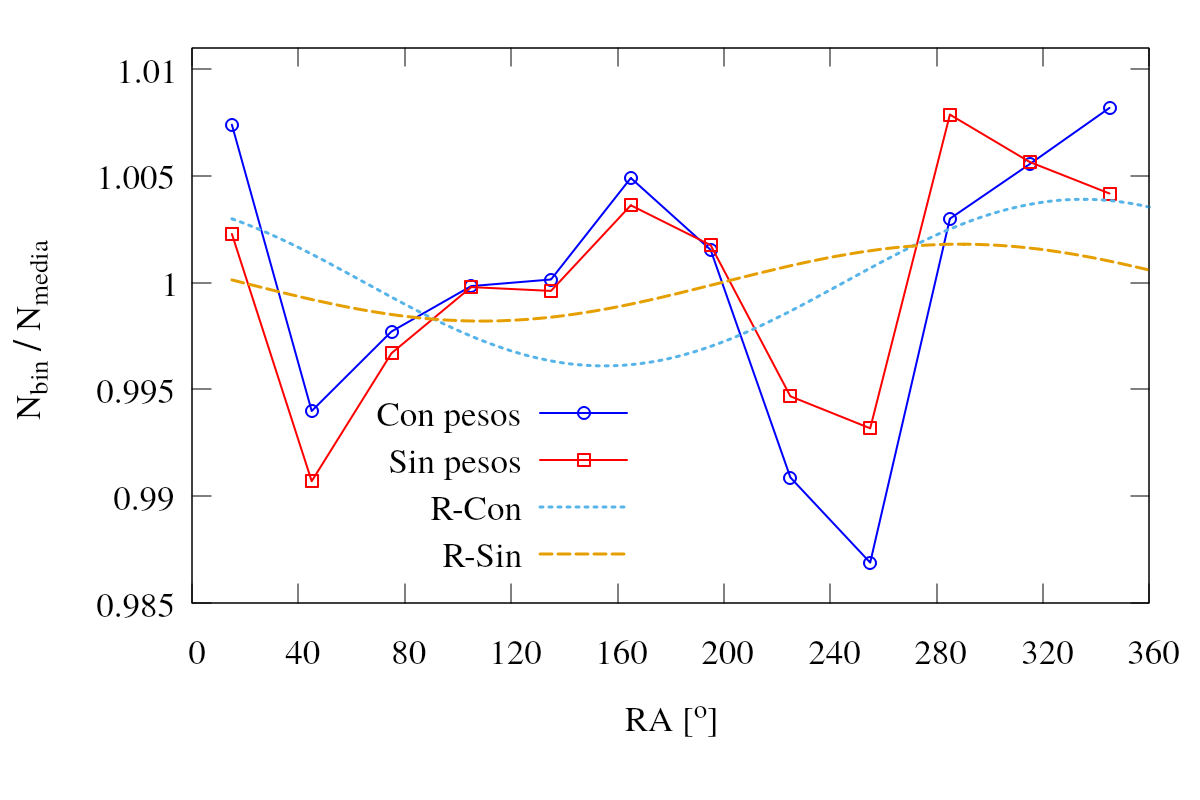
\includegraphics[width=0.75\linewidth]{eventos_clasificados_por_RA_v4.png}
		\caption{Distribución de la cantidad relativa de eventos en función de la ascensión recta a primer orden.}
	\end{figure}

	\begin{figure}[H]
		\centering
		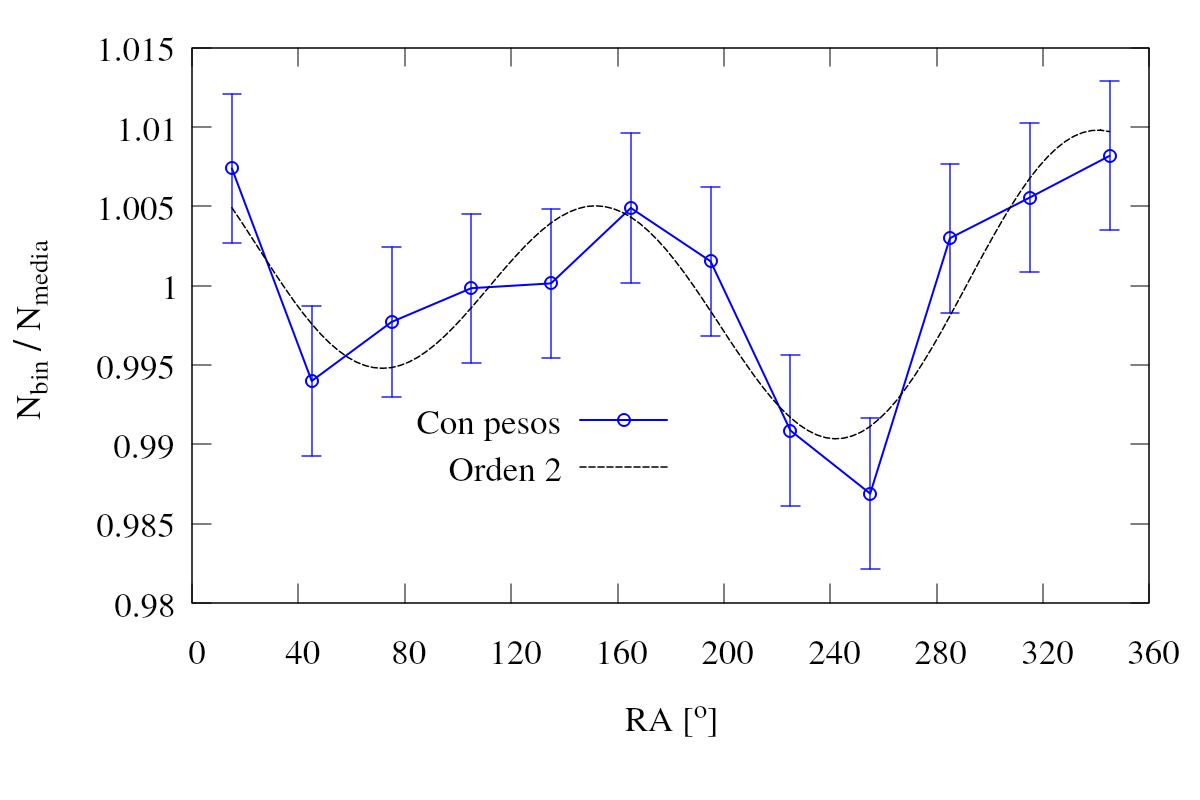
\includegraphics[width=0.75\linewidth]{eventos_clasificados_por_RA_v6_orden_2.png}
		\caption{Distribución de la cantidad relativa de eventos en función de la ascensión recta a segundo orden.}
	\end{figure}


La Figura 5.15 muestra la tasa de eventos normalizada en este intervalo de energía.
La línea continua es el valor del primer armónico obtenido a través del análisis de
Fourier. Es evidente que la modulación tiene características adicionales a las del primer
armónico, de hecho, el siguiente modo en valor de la amplitud es el cuarto, para el cual
$r 4 \alpha = 4.9 \times 10 -3 $con una probabilidad $P (>= r 4 \alpha ) = 2.7 \times 10 -3$ . La línea discontinua
muestra la distribución proveniente de la suma de los cuatro primeros armónicos. Es
interesante que el mayor exceso con respecto al caso dipolar es un salto en el intervalo
de ascensión recta $[ 270 ^o , 300 ^o ]$, muy cerca a la dirección del centro galáctico. Estudios
futuros de esta característica podrían ser interesantes para determinar su origen.

%%%%%%%%%%%%%%%%%%%%%%%%%5555

%%%%%%%%%%%%%%%%%%%%%%%%5

%%%%%%%%%%%%%%%%%%%%%%%%



% \begin{table}[H]
% \centering
% \begin{tabular}{l|c|c|c|c}
% 				& Con Peso 		& Sin peso 		& Con Peso 		& Sin peso 		\\ \hline
% Frecuencia:		& 366.21 		& 366.21 		& $\sim$366.505 & 366.506 		\\
% Fase:			& 151.032 		& 121.695		& $\sim$190 	& 73.8188		\\
% $P(r)$:		   & 0.289882\%	  & 46.9691 \% 	& $\sim$96\%	& 0.24013 \% 	\\
% Amplitud:		& 0.00512146	& 0.0018417		& $\sim$0.0006	& 0.00520328	\\
% \end{tabular}
% \caption{Fase, $r_{99}$ y $P_{99}$ del análisis de anisotropía entre en 1 de Enero del 2014 y el 1 de Enero del 2020}
% \label{tabla:pico}
% \end{table}






% \chapter{Modulación del clima para todos los disparos (2014-2020)}
% \graphicspath{{4_Weather_Modulation/}}
% 

La selección de los eventos genera dos conjuntos de datos: uno para el análisis de anisotropía en el bin 1 EeV - 2 EeV, y el segundo de los eventos con energía mayor a 1 Eev para obtener los parámetros del clima. En esta selección se tiene en cuentan los eventos de $\theta < 60^o$ , como también  los mismos que no se encuentren en un periodo de mala adquisición datos, este parámetro se denomina $ib$ de los \textbf{eventos del herald}. Este periodo consiste en momento donde el obsevatorio no recibe datos de las estaciones de clima o de los hexágonos. 

El parámetro de $ib$ de los \textbf{datos del clima} es irrelevante durante el proceso de filtrar eventos. Entra en juego cuando hago el análisis del clima, donde desecho los eventos que fueron recabados durante \emph{bad weather} \textbf{y} no fueron filtrados ya antes. 


\section{Pesos de los hexágonos}

Para constatar que no exista ninguna anomalía en los pesos de los hexágonos, se realiza el cálculo de los mismos para tres frecuencias de referencia para el análisis de anisotropías.  Los pesos se muestran en la Fig.\,\ref{fig:wei_14_20}. El rango de tiempo en el que se calculan estas curvas es entre 1 de Enero del 2014 y el 1 de Enero del 2020.

\begin{figure}[H]
	\centering
	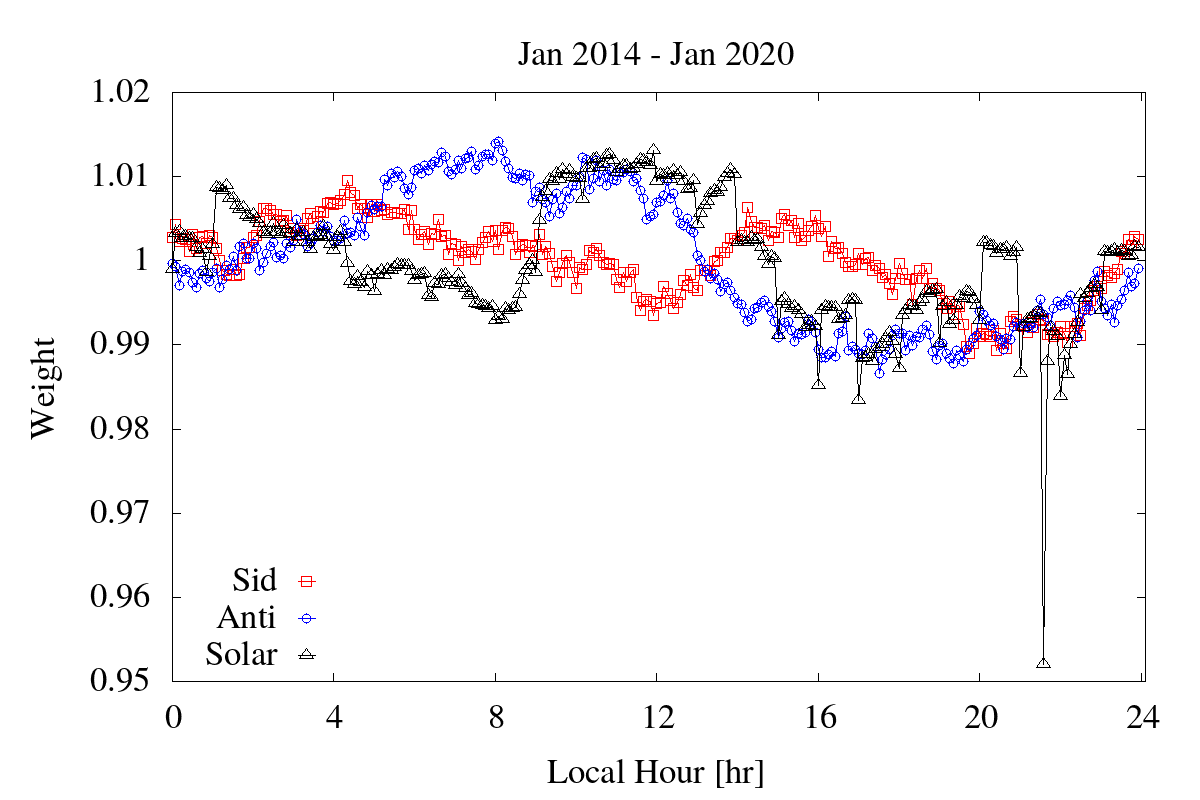
\includegraphics[width=0.5\textwidth]{weigth2014-2020_jan.png} 	
	\caption{Pesos de los hexágonos}
	\label{fig:wei_14_20}
\end{figure}

\section{Anisotropía}
El archivo de de todos los disparon empieza el Mon, 1 July 2013 12:05:08 GMT \footnote{$1372680308$}. Para trabajar en una cantidad entera de años, se trabaja a partir del  Thur, 1 January 2014 12:00:00 GMT \footnote{$1388577600$} y hasta el Thursday, 1 January 2020 12:00:00 GMT \footnote{$1577880000$}.  En este rango se tiene la tasa de eventos por día que se muestra en la Fig.\,\ref{tasa_total_diaria}.

% En el rango $1372680308$ \footnote{Mon, 1 July 2013 12:05:08 GMT} y $1388577600$ \footnote{Thur, 1 January 2014 12:00:00 GMT}, la tasa de eventos del archivo $\text{All Triggers}$, tenía una tasa de eventos por debajo de lo normal. Por esto, se utiliza los eventos a partir del  1388577600. La tasa de eventos que se utiliza se puede ver a continuación:

\begin{figure}[H]
	\centering
	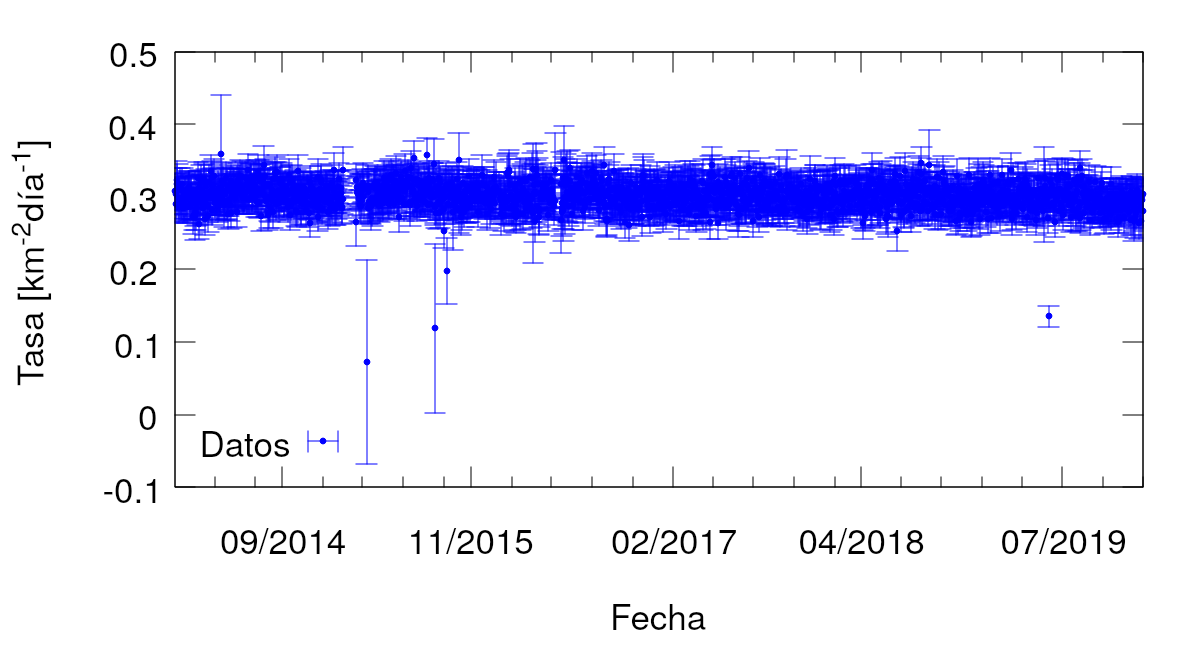
\includegraphics[width=0.5\textwidth]{rate_total.png}
	\caption{Tasa  de eventos en el rango de tiempo a trabajar}
	\label{tasa_total_diaria}
\end{figure}

\subsection{Lista detallada de los filtros aplicados de datos del herald}

\subsubsection{Datos para el análisis de anisotropía}
Esta sección muestra los filtros para los datos del análisis de anisotropía en el rango 1 EeV - 2 EeV.

\begin{enumerate}
	\item Energía entre  [1 EeV , 2 EeV)
	\item Rango de tiempo:
	\begin{itemize}
		\item[-] Inicial:1388577600 \\ (Thursday, 1 January 2014 12:00:00 GMT)
		\item[-] Final: 1577880000  \\ (Thursday, 1 January 2020 12:00:00 GMT)
	\end{itemize}
	\item Sectancia:  $\theta < 60^o$
	\item 6T5
	\item $ib=1$ Bad period flag. Un valor de 1 indica un buen periodo
\end{enumerate}

Con estos filtros se tienen $1\,092\,753$ eventos

\subsubsection{Datos para el cálculo de las correcciones del clima}

Estos son los filtros para los datos a utilizar para el cálculo de los parámetros del clima:

\begin{enumerate}
	\item Eventos con valor de señal de $S_{38}$\footnote{Valor de S38 sin la correccón del clima del paper del 2017} por encima de  $5.36\,\text{VEM}$. Este valor corresponde a $\sim 1\,$ EeV  en VEM.
	\item Rango de tiempo:
	\begin{itemize}
		\item[-] Inicial:1388577600 \\ (Thursday, 1 January 2014 12:00:00 GMT)
		\item[-] Final: 1577880000  \\ (Thursday, 1 January 2020 12:00:00 GMT)
	\end{itemize}
	\item Sectancia:  $\theta < 60^o$
	\item $iw<4$ (weather quality flag)
	\item 6T5
	\item $ib=1$ Bad period flag del herald.  Un valor de 1 indica un buen periodo
	\item $ib=1$ Bad period flag de los datos del clima. Un valor de 1 indica un buen periodo
\end{enumerate}


Con estos filtros se tienen $1\,208\,615$ eventos, con una tasa de eventos que se muestra en la Fig.\,\ref{tasa_total_diaria_ajuste_weather}. En la figura se observa que utilizando el corte en la señal de S38 sin corregir por la modulación del clima del herald \footnote{Las correcciones se calcularon para el archivo del disparo estándar} se observa una modulación anual.

\begin{figure}[H]
	\centering
	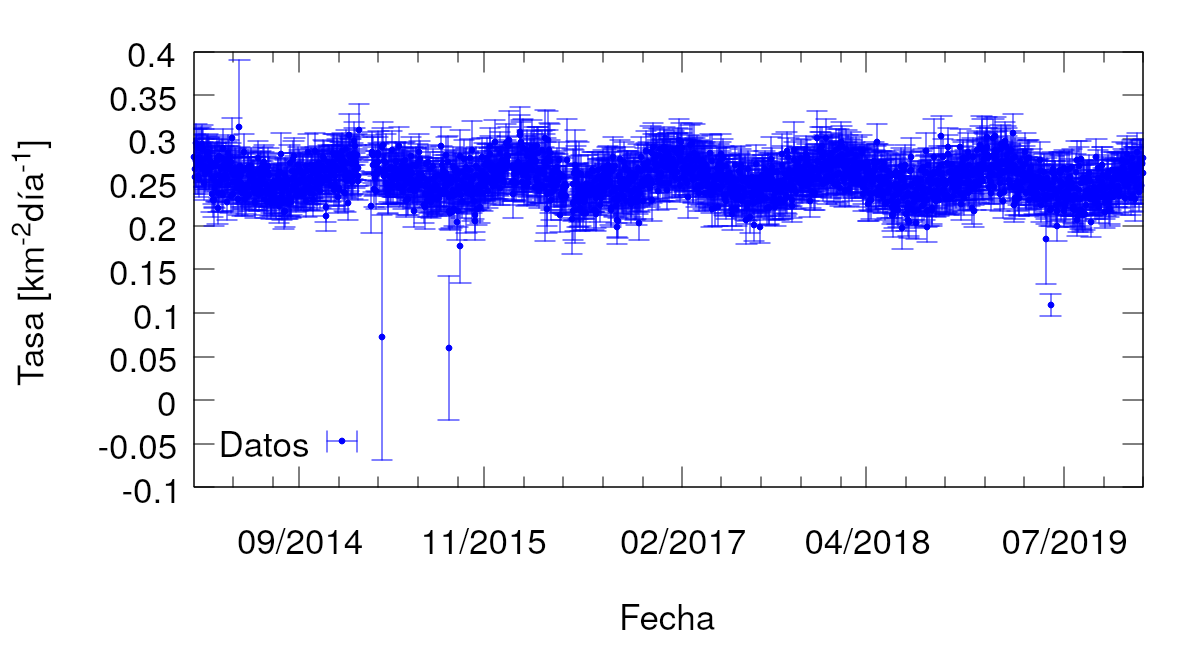
\includegraphics[width=0.5\textwidth]{rate_total_ajuste_weather.png}
	\caption{Tasa  de eventos en el rango de tiempo a trabajar para el ajuste de los parámetros del clima.}
	\label{tasa_total_diaria_ajuste_weather}
\end{figure}


\subsection{Análisis en frecuencia}

\begin{figure}[H]
	\centering
	\includegraphics[width=0.5\textwidth]{2019_AllTriggers_1_2_EeV_con_vs_sin_peso.png}
	\caption{Análisis en frecuencia en ascensión recta en rango 1 EeV - 2 EeV}
	\label{fig:consin}
\end{figure}


\section{Corrección del clima}

\begin{figure}[H]
	\centering
	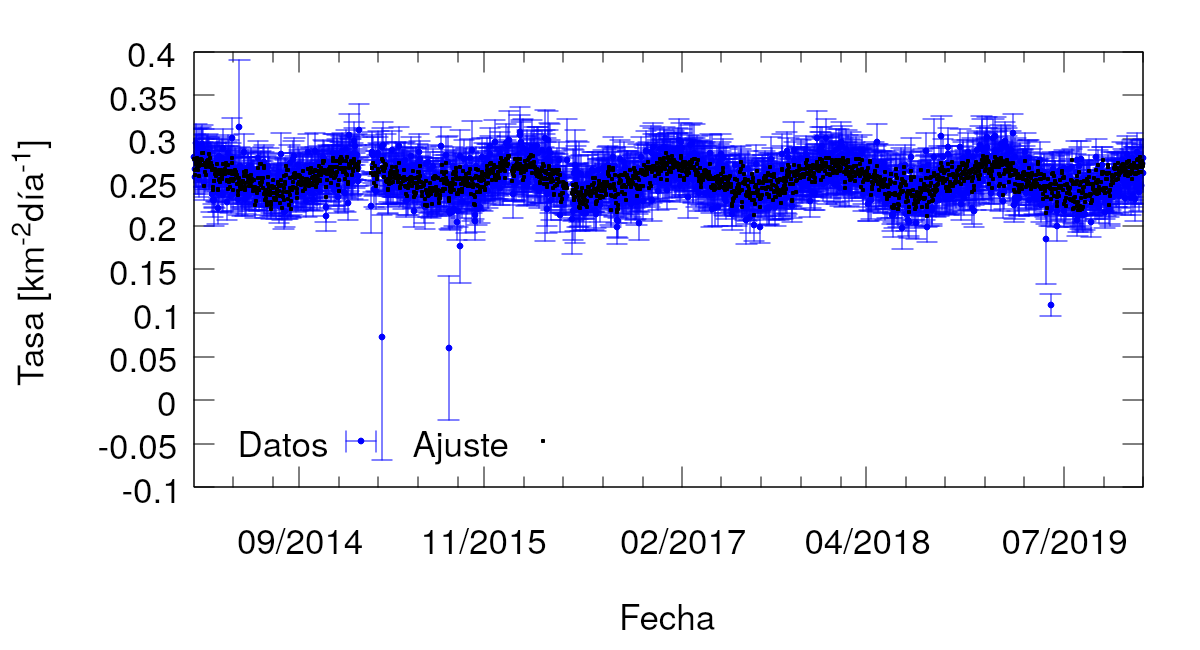
\includegraphics[width=0.5\textwidth]{rate_Ajuste.png}
\end{figure}

%%%%%%%%5
\begin{figure}[H]
\begin{subfigure}{.5\textwidth}
	\centering
	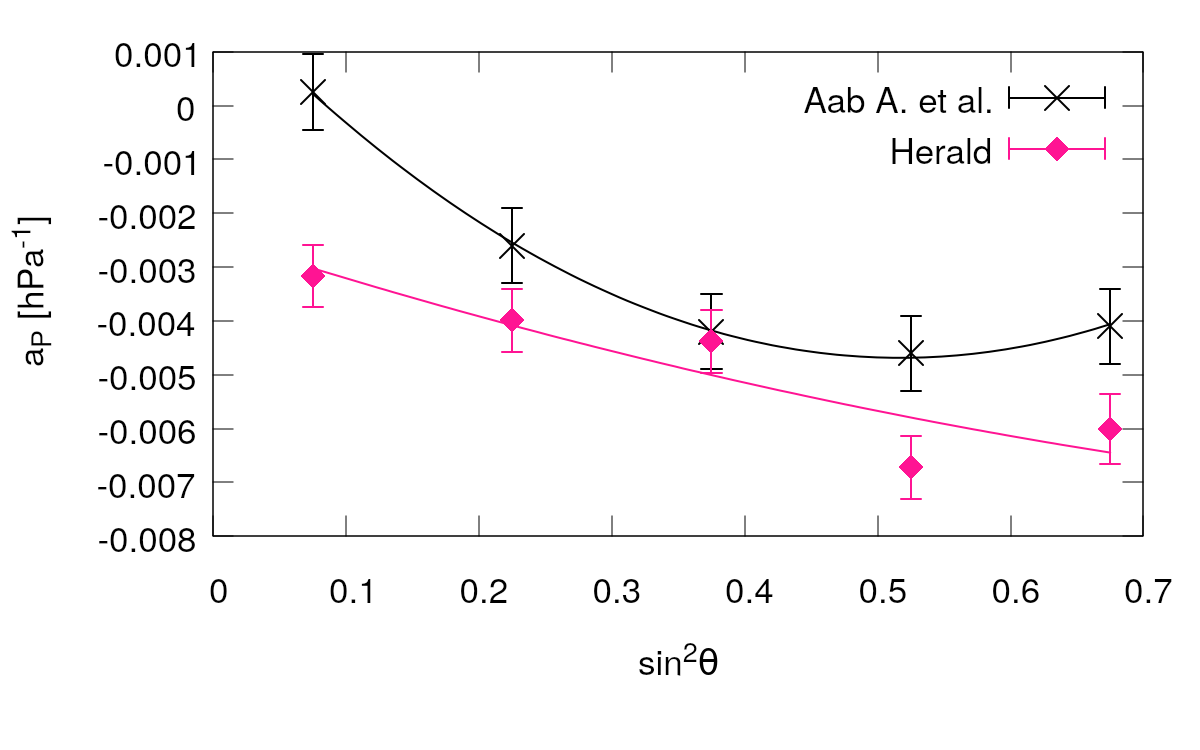
\includegraphics[width=\linewidth]{ap_6t5.png}
	\caption{Parámetro de clima $a_P$}
\end{subfigure}%
\begin{subfigure}{.5\textwidth}
	\centering
	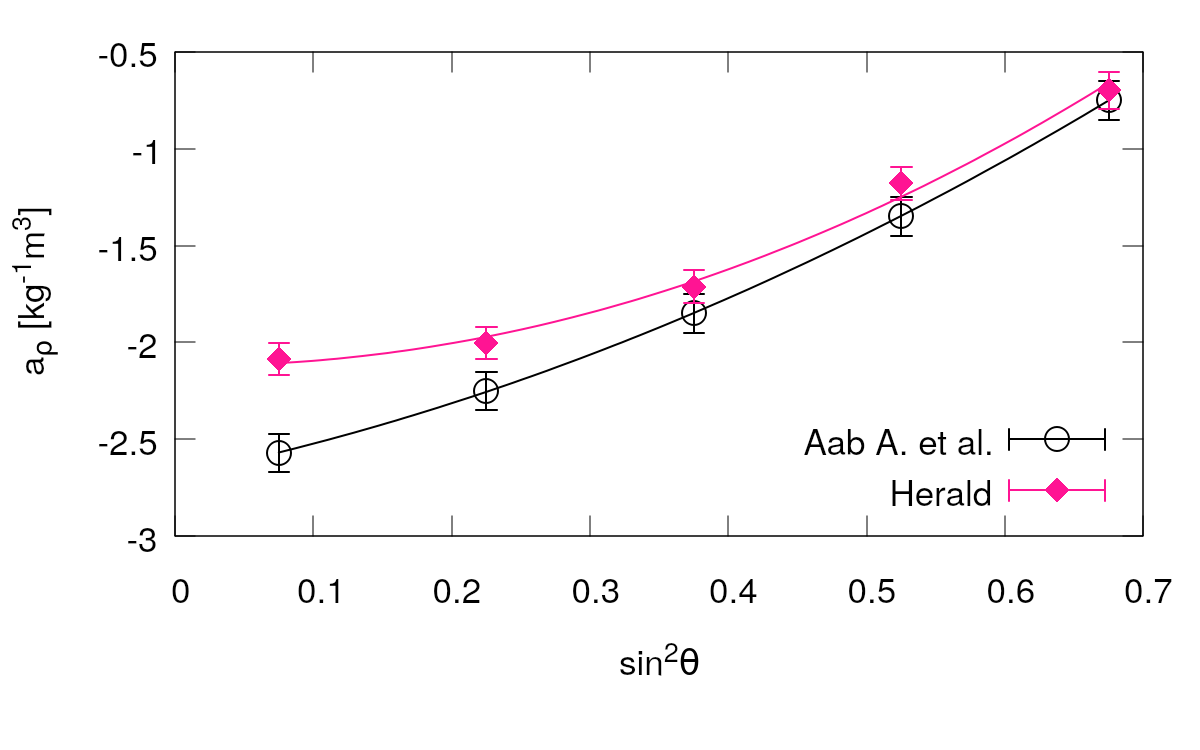
\includegraphics[width=\linewidth]{arho_6t5.png}
	\caption{Parámetro de clima $a_\rho$}
\end{subfigure}\\
\centering
\begin{subfigure}{.5\textwidth}
	\centering
	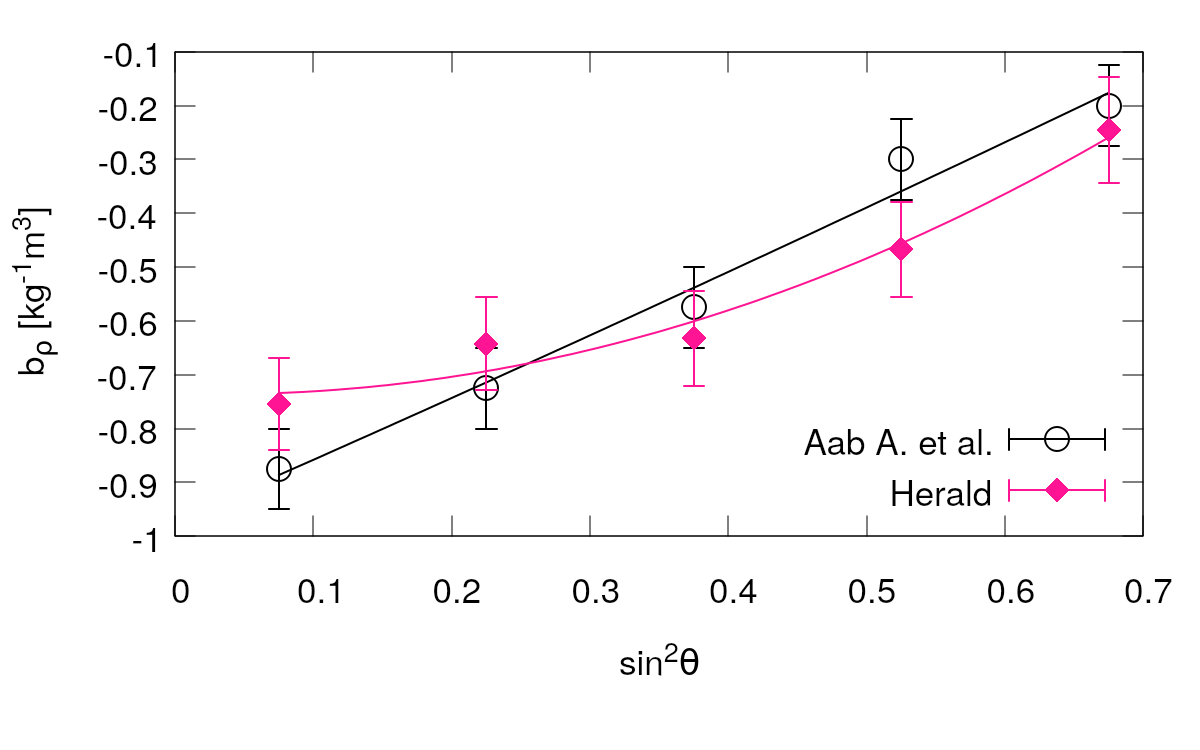
\includegraphics[width=\linewidth]{brho_6t5.png}
	\caption{Parámetro de clima $b_\rho$}
\end{subfigure}%
\caption{Parámetros de clima calculados para la corrección del archivo de todos los disparos}
\end{figure}
%%%%%%%%


%%%%%%%%%%%%%%%%%%%%%%%%%%%%%%%%%%%%%%%%%%%%%%%%%%%%%%%%%%%%%%%%%%%%%%%%%%%%%%%%%%%%%%%%%
%%%%%%%%%%%%%%%%%%%%%%%%%%%%%%%%%%%%%%%%%%%%%%%%%%%%%%%%%%%%%%%%%%%%%%%%%%%%%%%%%%%%%%%%%
%%%%%%%%%%%%%%%%%%%%%%%%%%%%%%%%%%%%%%%%%%%%%%%%%%%%%%%%%%%%%%%%%%%%%%%%%%%%%%%%%%%%%%%%%

      \subsubsection{Modulación del clima para todos los triggers}

      Para corroborar los parámetros del clima, primero calculé las tasas de eventos de los archivos del 2017 y 2020 para energías mayores a 1  EeV, donde obtuve los siguientes gráficos Fig.\ref{fig:rate_daily_2017_1EeV} y \ref{fig:rate_daily_2020_1EeV}. 

        \begin{figure}[H]
        
          \begin{subfigure}[b]{0.5\textwidth}
          \centering
          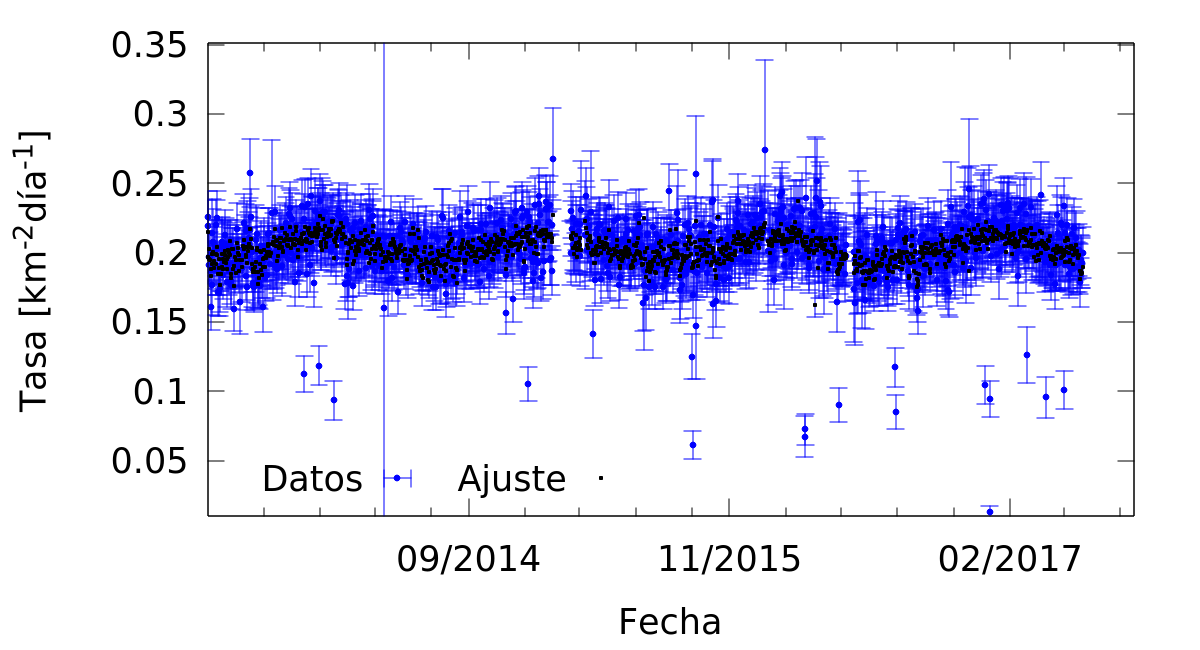
\includegraphics[width=\textwidth]{../IntroduccionReport/daily_rate/daily_rate_AllTriggers_2017_1EeV.png}
          \caption{Archivo de 2017}   \label{fig:rate_daily_2017_1EeV}
          \end{subfigure}%
        \hfill
          \begin{subfigure}[b]{0.5\textwidth}
          \centering
          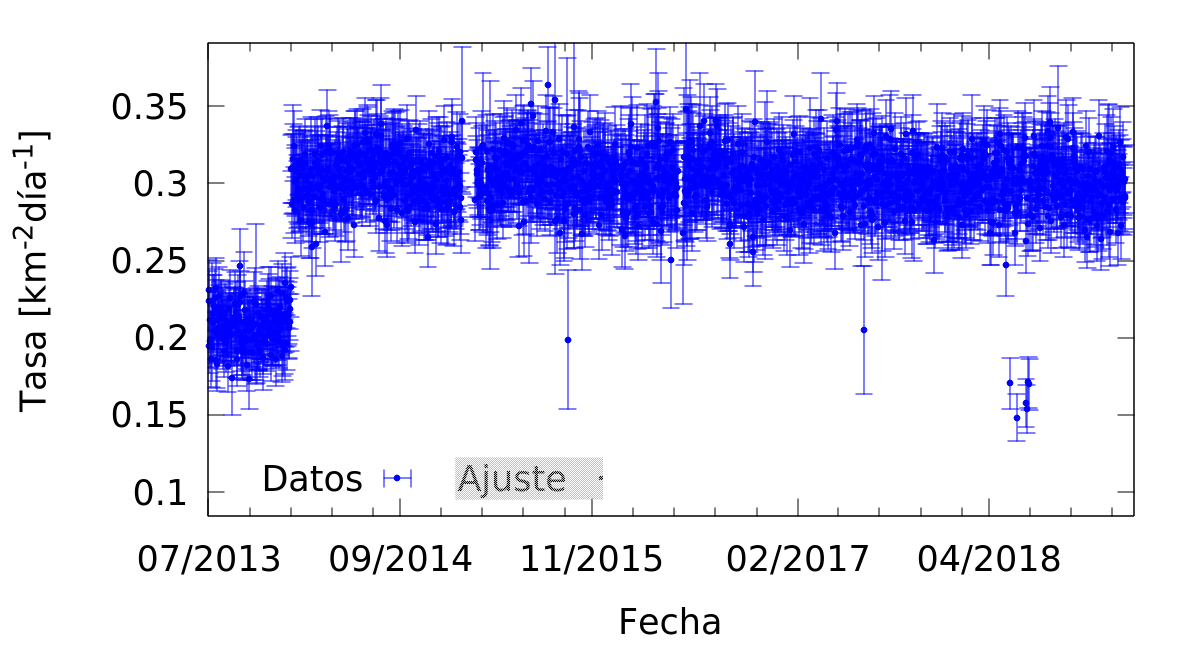
\includegraphics[width=\textwidth]{../IntroduccionReport/daily_rate/daily_rate_AllTriggers_2019_1EeV.png}
          \caption{Archivo del 2020}  \label{fig:rate_daily_2020_1EeV}
          \end{subfigure}
          \caption{Tasa de eventos diaria por encima de 1 EeV para los datos de todos los disparos.}
        \end{figure}

      Después calculé los parámetros del clima para energía mayores a 1 EeV. Para el archivo de 2017 obtuve la Fig.\,\ref{fig:parameters_2017_1EeV}. Los comparé con el paper del weather del main array, para ver si dan algo razonable. Verifiqué las siguientes cosas para el ajuste

      \begin{itemize}
        \item Me fijé que delay en la densidad cada momento fuera de dos  horas
        \item Me fijé que el ajuste no tuviera en cuenta periodos malos, bad periods
        \item Me fijé que el delay de la densidad media también fuera tal que para cada evento estuviera centrada $\pm$12 horas
        \item También me fijé que el rango de tiempo estuviera bien, porque estos datos están disponibles desde el 2013  recién
        \item Me fijé que los $\chi^2$ reducido fuera algo razonable. Todos rondaban alrededor de $1.05$
      \end{itemize}

      EL rango de tiempo que usé fue este: 
      \begin{itemize}
        \item Inicio: 1372680308
        \item Final: 1496275090
      \end{itemize}
        \begin{figure}[H]
          \begin{subfigure}[b]{0.5\textwidth}
          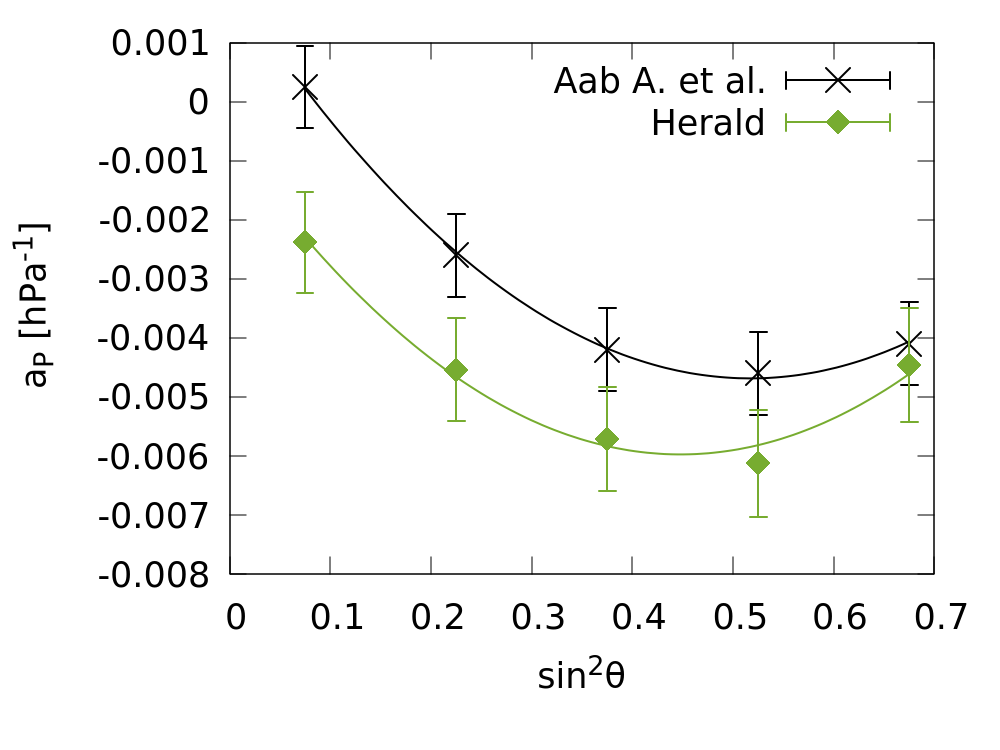
\includegraphics[width=\linewidth]{../IntroduccionReport/params/ap_2017_above_1EeV.png}
          \caption{Parámetro $a_P$ }
          \label{fig:ap_2017_1EeV}
          \end{subfigure}%
          \hspace{\fill}
          \begin{subfigure}[b]{0.5\textwidth}
          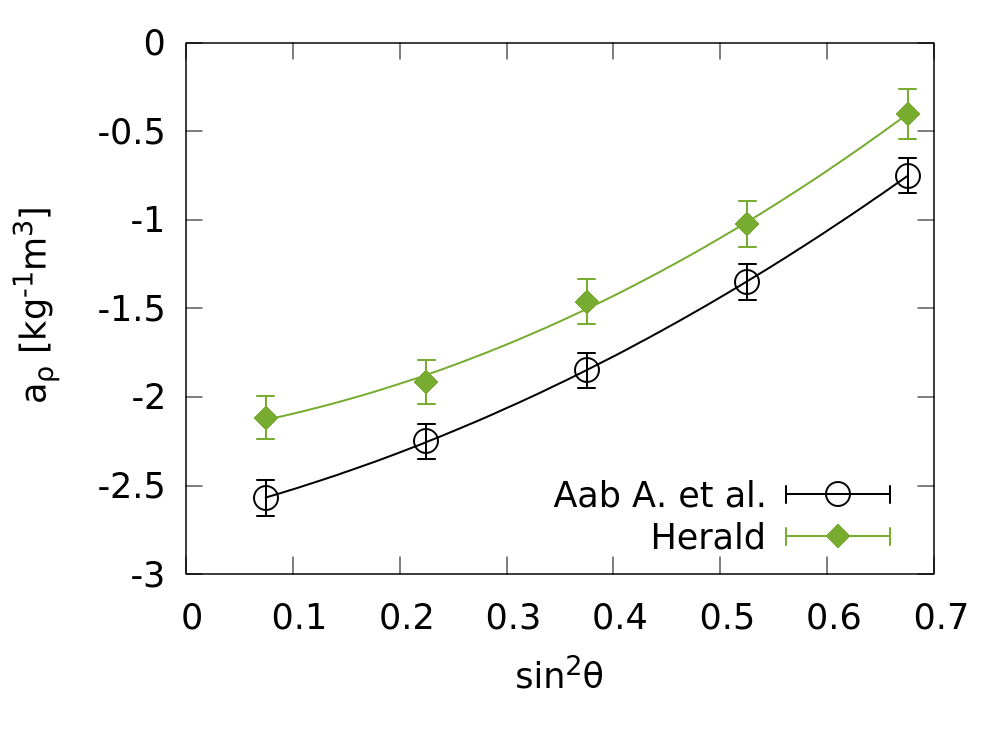
\includegraphics[width=\linewidth]{../IntroduccionReport/params/arho_2017_above_1EeV.png}
          \caption{Parámetro $a_{\rho}$ }
          \label{fig:arho_2017_1EeV}
          \end{subfigure}%
          \hspace{\fill}
          \begin{subfigure}[b]{\textwidth}
          \centering
          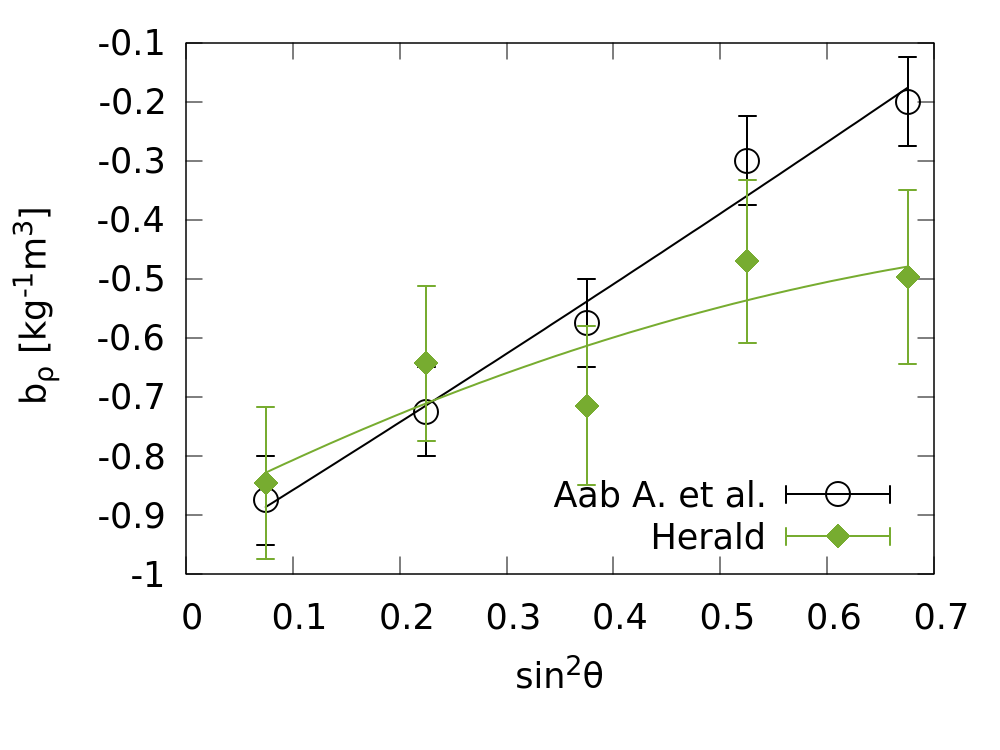
\includegraphics[width=0.5\linewidth]{../IntroduccionReport/params/brho_2017_above_1EeV.png}
          \caption{Parámetro  $b_\rho$   }
          \label{fig:brho_2017_1EeV}
          \end{subfigure}%
          \caption{Parámetros de la modulación del clima considerando los datos para todos los disparos de 2017. Los mismos se comparan con los ajustes obtenidos en \cite{aab2017impact}.}\label{fig:parameters_2017_1EeV}
        \end{figure}

        Lo que más me llama la atención es el comportamiento del parámetro $b_\rho$, que como se discutió en otras oportunidades, tiene que ver con el parámetro $a_\rho$ con una razón de  $1:3$ más o menos. 



      Hacemos el mismo procedimiento con el archivo 2020, {\bf pero filtrando los eventos por el valor de S38 sin corregir por la modulación del clima}. Para calcular la tasa y los parámetros del clima, se toman los eventos después de ese salto de 0.2 a 0.3, obtengo los siguientes resultados:

        \begin{figure}[H]
          \centering
          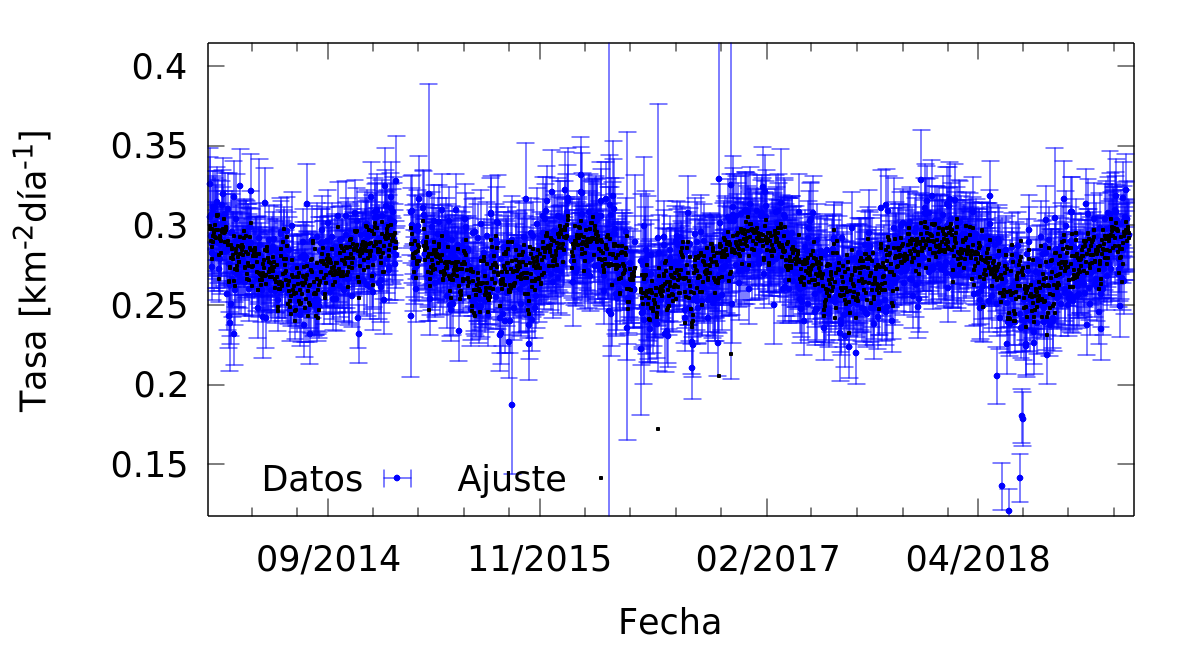
\includegraphics[width=0.5\textwidth]{../IntroduccionReport/daily_rate/daily_rate_AllTriggers_2020_1EeV.png}
        \end{figure}

      Acá también verifiqué lo mismo que el caso anterior, lo único que ahora el $\chi^2$ rondaba alrededor de los $1.08$. Siempre verifico que no sea mucho mayor o menor a 1.

      EL rango de tiempo que usé para este caso fue este: 
      \begin{itemize}
        \item Inicio: 1388910508
        \item Final: 1550490858
      \end{itemize}
      
        \begin{figure}[H]
          \begin{subfigure}[b]{0.5\textwidth}
          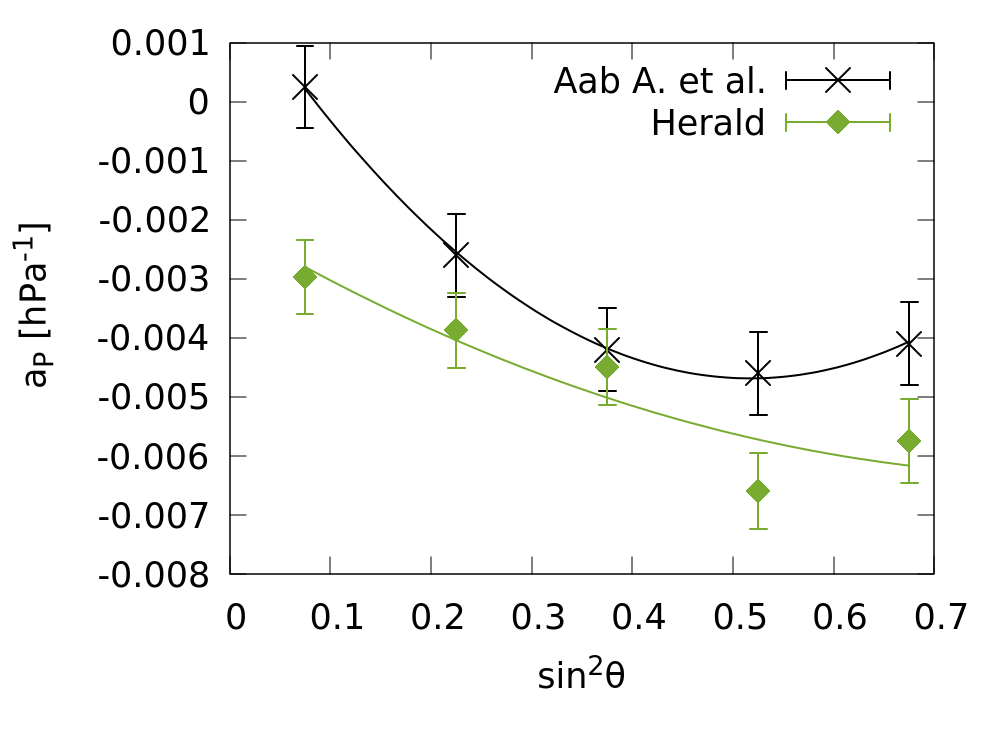
\includegraphics[width=\linewidth]{../IntroduccionReport/params/ap_2020_above_1EeV.png}
          \caption{Parámetro $a_P$ }
          \label{fig:ap_2020_1EeV}
          \end{subfigure}%
          \hspace{\fill}
          \begin{subfigure}[b]{0.5\textwidth}
          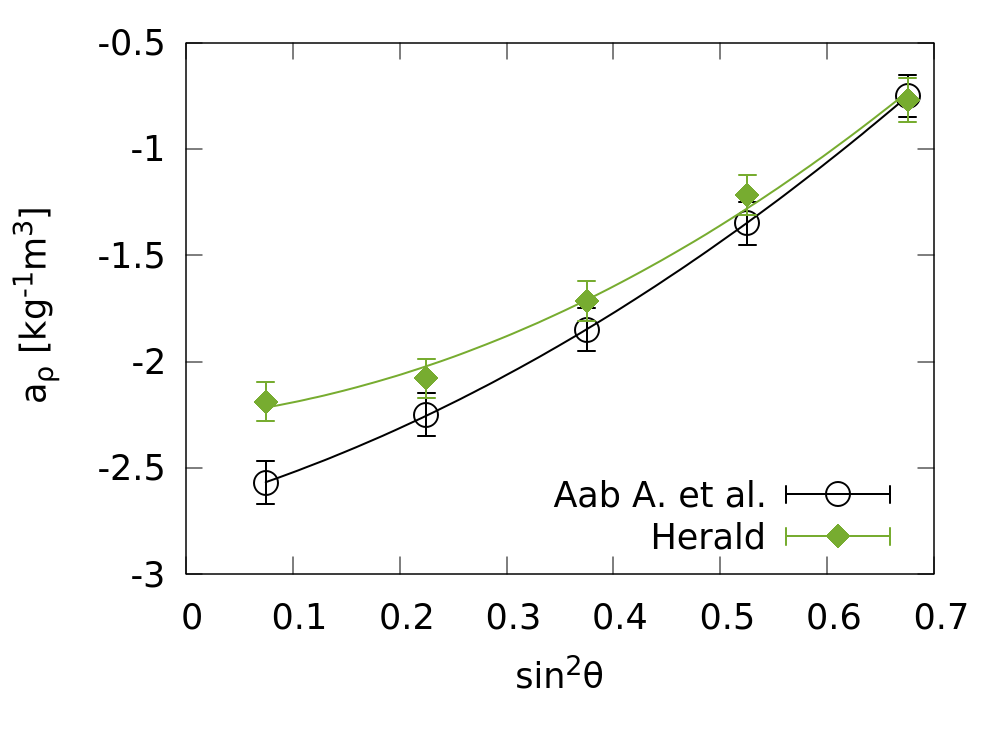
\includegraphics[width=\linewidth]{../IntroduccionReport/params/arho_2020_above_1EeV.png}
          \caption{Parámetro $a_{\rho}$ }
          \label{fig:arho_2020_1EeV}
          \end{subfigure}%
          \hspace{\fill}
          \begin{subfigure}[b]{\textwidth}
          \centering
          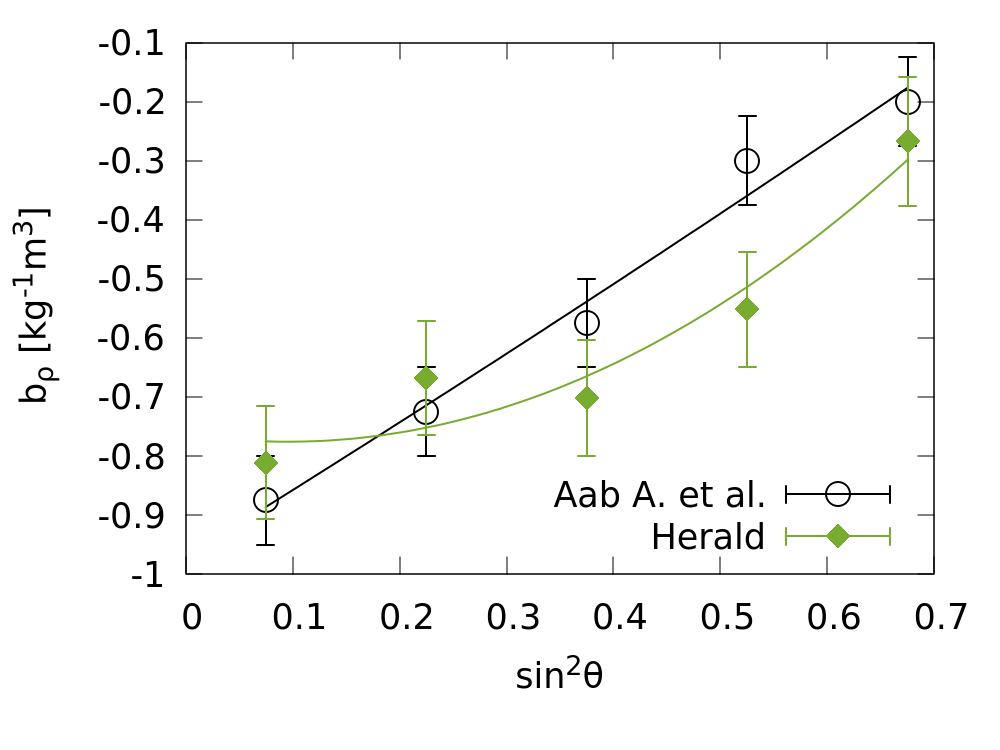
\includegraphics[width=0.5\linewidth]{../IntroduccionReport/params/brho_2020_above_1EeV.png}
          \caption{Parámetro  $b_\rho$   }
          \label{fig:brho_2020_1EeV}
          \end{subfigure}%
          \caption{Parámetros de la modulación del clima considerando los datos para todos los disparos de 2020. Los mismos se comparan con los ajustes obtenidos en \cite{aab2017impact}.}\label{fig:parameters_2020_1EeV}
        \end{figure}



      Considerando el filtro con el S38 en el archivo 2020 y la energía en el 2017, quiero saber si obtengo parametros  del clima comparables. Ya que el Main Array se corresponden los parametros del 2015 y 2019, yo esperaría que con todos los triggers pase los mismo. Una diferencia importante entre ambos análisis es que los parametros del 2020 contienen eventos hasta el 31/12/2019.


        \begin{figure}[H]
          \begin{subfigure}[b]{0.5\textwidth}
          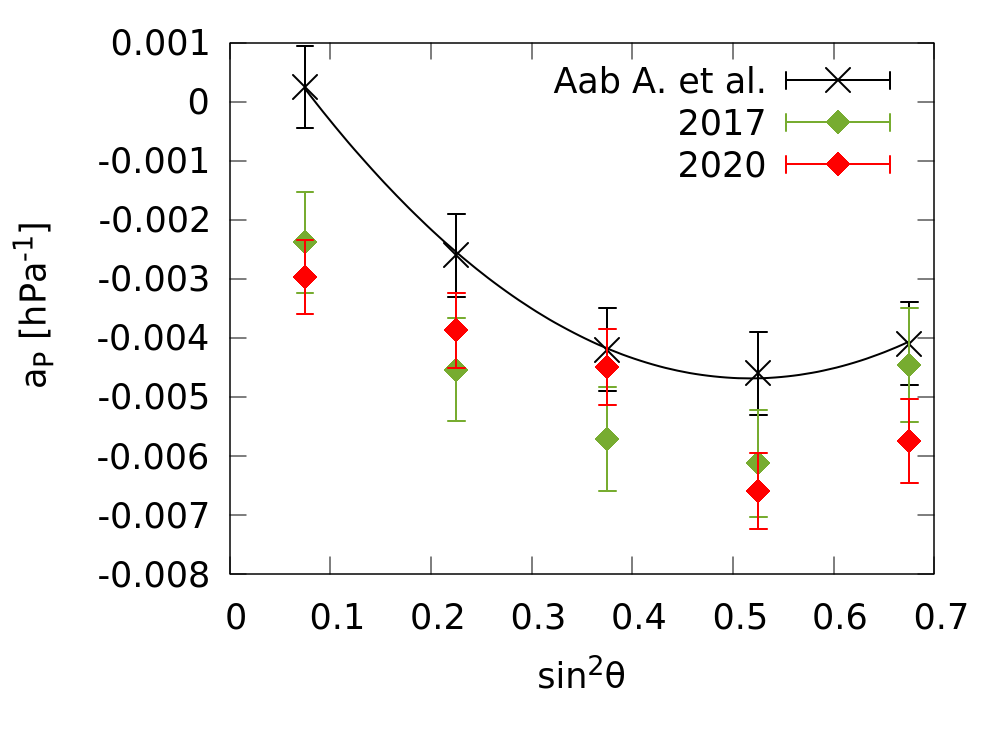
\includegraphics[width=\linewidth]{../IntroduccionReport/params/ap_2017_2020_above_1EeV.png}
          \caption{Parámetro $a_P$ }
          \end{subfigure}%
          \hspace{\fill}
          \begin{subfigure}[b]{0.5\textwidth}
          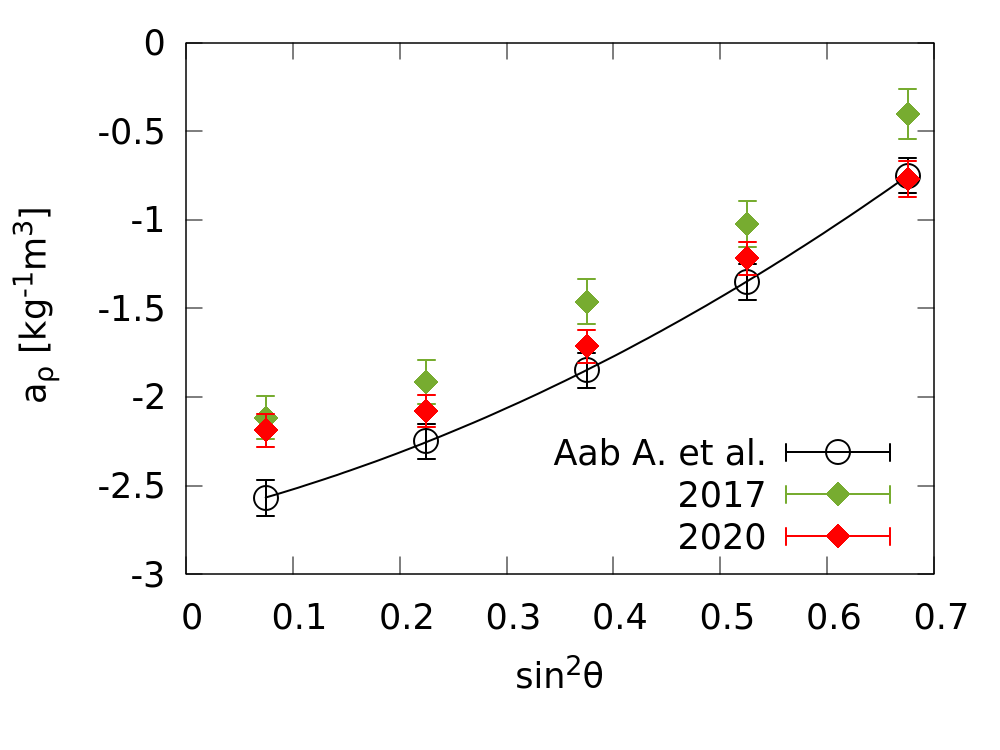
\includegraphics[width=\linewidth]{../IntroduccionReport/params/arho_2017_2020_above_1EeV.png}
          \caption{Parámetro $a_{\rho}$ }
          \end{subfigure}%
          \hspace{\fill}
          \begin{subfigure}[b]{\textwidth}
          \centering
          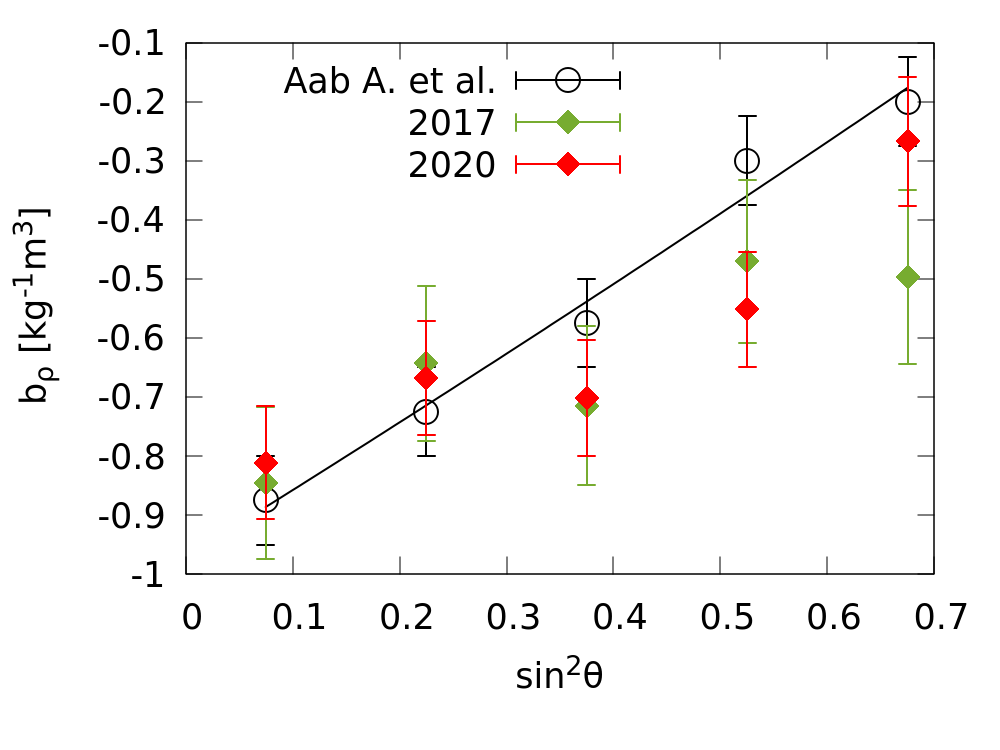
\includegraphics[width=0.5\linewidth]{../IntroduccionReport/params/brho_2017_2020_above_1EeV.png}
          \caption{Parámetro  $b_\rho$   }
          \end{subfigure}%
          \caption{Parámetros de la modulación del clima considerando los datos para todos los disparos del archivo 2017 y 2020. Los mismos se comparan con los ajustes obtenidos en \cite{aab2017impact}.}
        \end{figure}

      Se ve que estos parámetros no son comparables. 



\begin{biblio}
	\bibliography{mibib}
\end{biblio}



\end{document}